\documentclass[1p]{elsarticle_modified}
%\bibliographystyle{elsarticle-num}

%\usepackage[colorlinks]{hyperref}
%\usepackage{abbrmath_seonhwa} %\Abb, \Ascr, \Acal ,\Abf, \Afrak
\usepackage{amsfonts}
\usepackage{amssymb}
\usepackage{amsmath}
\usepackage{amsthm}
\usepackage{scalefnt}
\usepackage{amsbsy}
\usepackage{kotex}
\usepackage{caption}
\usepackage{subfig}
\usepackage{color}
\usepackage{graphicx}
\usepackage{xcolor} %% white, black, red, green, blue, cyan, magenta, yellow
\usepackage{float}
\usepackage{setspace}
\usepackage{hyperref}

\usepackage{tikz}
\usetikzlibrary{arrows}

\usepackage{multirow}
\usepackage{array} % fixed length table
\usepackage{hhline}

%%%%%%%%%%%%%%%%%%%%%
\makeatletter
\renewcommand*\env@matrix[1][\arraystretch]{%
	\edef\arraystretch{#1}%
	\hskip -\arraycolsep
	\let\@ifnextchar\new@ifnextchar
	\array{*\c@MaxMatrixCols c}}
\makeatother %https://tex.stackexchange.com/questions/14071/how-can-i-increase-the-line-spacing-in-a-matrix
%%%%%%%%%%%%%%%

\usepackage[normalem]{ulem}

\newcommand{\msout}[1]{\ifmmode\text{\sout{\ensuremath{#1}}}\else\sout{#1}\fi}
%SOURCE: \msout is \stkout macro in https://tex.stackexchange.com/questions/20609/strikeout-in-math-mode

\newcommand{\cancel}[1]{
	\ifmmode
	{\color{red}\msout{#1}}
	\else
	{\color{red}\sout{#1}}
	\fi
}

\newcommand{\add}[1]{
	{\color{blue}\uwave{#1}}
}

\newcommand{\replace}[2]{
	\ifmmode
	{\color{red}\msout{#1}}{\color{blue}\uwave{#2}}
	\else
	{\color{red}\sout{#1}}{\color{blue}\uwave{#2}}
	\fi
}

\newcommand{\Sol}{\mathcal{S}} %segment
\newcommand{\D}{D} %diagram
\newcommand{\A}{\mathcal{A}} %arc


%%%%%%%%%%%%%%%%%%%%%%%%%%%%%5 test

\def\sl{\operatorname{\textup{SL}}(2,\Cbb)}
\def\psl{\operatorname{\textup{PSL}}(2,\Cbb)}
\def\quan{\mkern 1mu \triangleright \mkern 1mu}

\theoremstyle{definition}
\newtheorem{thm}{Theorem}[section]
\newtheorem{prop}[thm]{Proposition}
\newtheorem{lem}[thm]{Lemma}
\newtheorem{ques}[thm]{Question}
\newtheorem{cor}[thm]{Corollary}
\newtheorem{defn}[thm]{Definition}
\newtheorem{exam}[thm]{Example}
\newtheorem{rmk}[thm]{Remark}
\newtheorem{alg}[thm]{Algorithm}

\newcommand{\I}{\sqrt{-1}}
\begin{document}

%\begin{frontmatter}
%
%\title{Boundary parabolic representations of knots up to 8 crossings}
%
%%% Group authors per affiliation:
%\author{Yunhi Cho} 
%\address{Department of Mathematics, University of Seoul, Seoul, Korea}
%\ead{yhcho@uos.ac.kr}
%
%
%\author{Seonhwa Kim} %\fnref{s_kim}}
%\address{Center for Geometry and Physics, Institute for Basic Science, Pohang, 37673, Korea}
%\ead{ryeona17@ibs.re.kr}
%
%\author{Hyuk Kim}
%\address{Department of Mathematical Sciences, Seoul National University, Seoul 08826, Korea}
%\ead{hyukkim@snu.ac.kr}
%
%\author{Seokbeom Yoon}
%\address{Department of Mathematical Sciences, Seoul National University, Seoul, 08826,  Korea}
%\ead{sbyoon15@snu.ac.kr}
%
%\begin{abstract}
%We find all boundary parabolic representation of knots up to 8 crossings.
%
%\end{abstract}
%\begin{keyword}
%    \MSC[2010] 57M25 
%\end{keyword}
%
%\end{frontmatter}

%\linenumbers
%\tableofcontents
%
\newcommand\colored[1]{\textcolor{white}{\rule[-0.35ex]{0.8em}{1.4ex}}\kern-0.8em\color{red} #1}%
%\newcommand\colored[1]{\textcolor{white}{ #1}\kern-2.17ex	\textcolor{white}{ #1}\kern-1.81ex	\textcolor{white}{ #1}\kern-2.15ex\color{red}#1	}

{\Large $\underline{12a_{0362}~(K12a_{0362})}$}

\setlength{\tabcolsep}{10pt}
\renewcommand{\arraystretch}{1.6}
\vspace{1cm}\begin{tabular}{m{100pt}>{\centering\arraybackslash}m{274pt}}
\multirow{5}{120pt}{
	\centering
	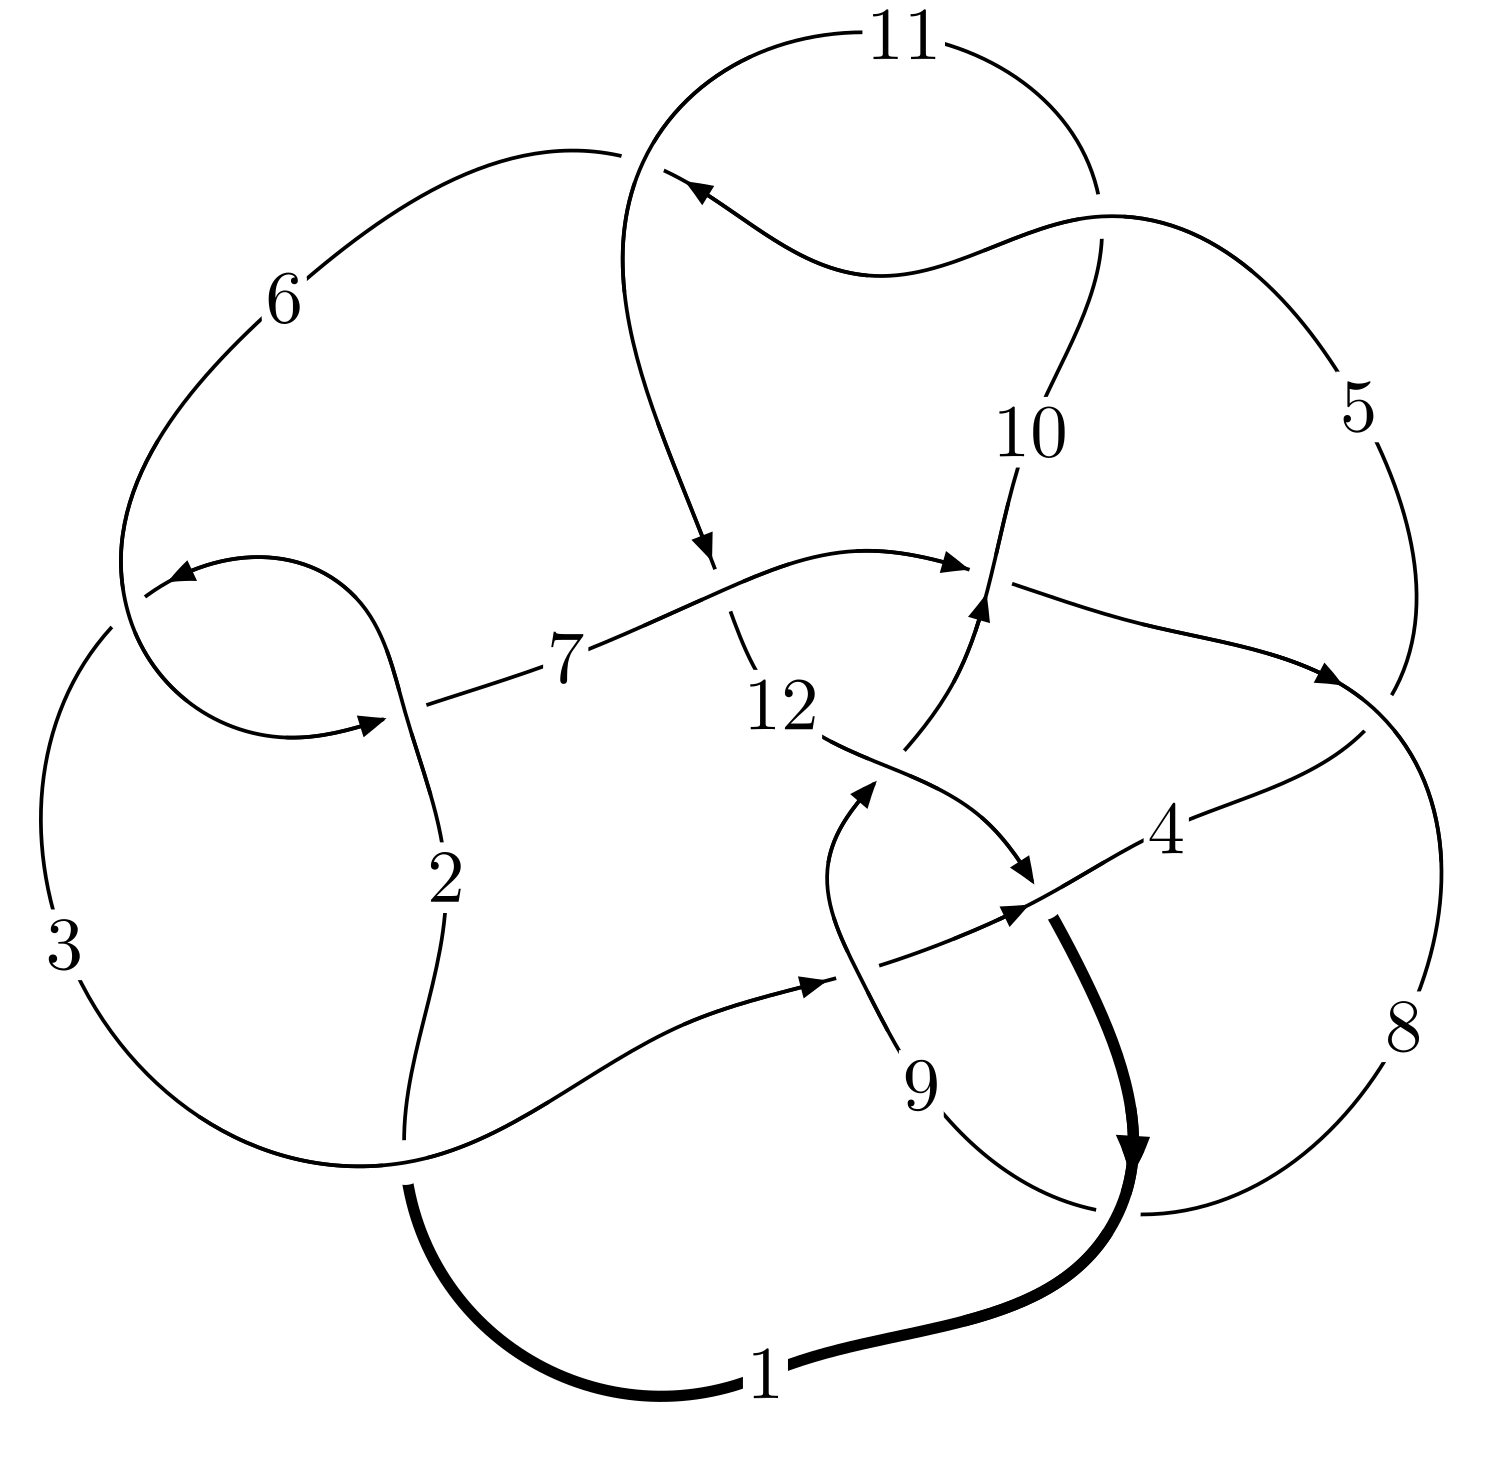
\includegraphics[width=112pt]{../../../GIT/diagram.site/Diagrams/png/1163_12a_0362.png}\\
\ \ \ A knot diagram\footnotemark}&
\allowdisplaybreaks
\textbf{Linearized knot diagam} \\
\cline{2-2}
 &
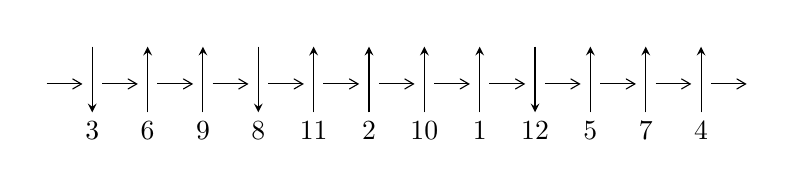
\begin{tikzpicture}[x=20pt, y=17pt]
	% nodes
	\node (C0) at (0, 0) {};
	\node (C1) at (1, 0) {};
	\node (C1U) at (1, +1) {};
	\node (C1D) at (1, -1) {3};

	\node (C2) at (2, 0) {};
	\node (C2U) at (2, +1) {};
	\node (C2D) at (2, -1) {6};

	\node (C3) at (3, 0) {};
	\node (C3U) at (3, +1) {};
	\node (C3D) at (3, -1) {9};

	\node (C4) at (4, 0) {};
	\node (C4U) at (4, +1) {};
	\node (C4D) at (4, -1) {8};

	\node (C5) at (5, 0) {};
	\node (C5U) at (5, +1) {};
	\node (C5D) at (5, -1) {11};

	\node (C6) at (6, 0) {};
	\node (C6U) at (6, +1) {};
	\node (C6D) at (6, -1) {2};

	\node (C7) at (7, 0) {};
	\node (C7U) at (7, +1) {};
	\node (C7D) at (7, -1) {10};

	\node (C8) at (8, 0) {};
	\node (C8U) at (8, +1) {};
	\node (C8D) at (8, -1) {1};

	\node (C9) at (9, 0) {};
	\node (C9U) at (9, +1) {};
	\node (C9D) at (9, -1) {12};

	\node (C10) at (10, 0) {};
	\node (C10U) at (10, +1) {};
	\node (C10D) at (10, -1) {5};

	\node (C11) at (11, 0) {};
	\node (C11U) at (11, +1) {};
	\node (C11D) at (11, -1) {7};

	\node (C12) at (12, 0) {};
	\node (C12U) at (12, +1) {};
	\node (C12D) at (12, -1) {4};
	\node (C13) at (13, 0) {};

	% arrows
	\draw[->,>={angle 60}]
	(C0) edge (C1) (C1) edge (C2) (C2) edge (C3) (C3) edge (C4) (C4) edge (C5) (C5) edge (C6) (C6) edge (C7) (C7) edge (C8) (C8) edge (C9) (C9) edge (C10) (C10) edge (C11) (C11) edge (C12) (C12) edge (C13) ;	\draw[->,>=stealth]
	(C1U) edge (C1D) (C2D) edge (C2U) (C3D) edge (C3U) (C4U) edge (C4D) (C5D) edge (C5U) (C6D) edge (C6U) (C7D) edge (C7U) (C8D) edge (C8U) (C9U) edge (C9D) (C10D) edge (C10U) (C11D) edge (C11U) (C12D) edge (C12U) ;
	\end{tikzpicture} \\
\hhline{~~} \\& 
\textbf{Solving Sequence} \\ \cline{2-2} 
 &
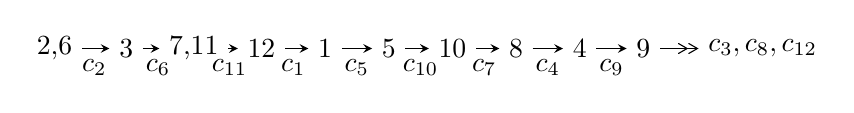
\begin{tikzpicture}[x=23pt, y=7pt]
	% node
	\node (A0) at (-1/8, 0) {2,6};
	\node (A1) at (1, 0) {3};
	\node (A2) at (33/16, 0) {7,11};
	\node (A3) at (25/8, 0) {12};
	\node (A4) at (33/8, 0) {1};
	\node (A5) at (41/8, 0) {5};
	\node (A6) at (49/8, 0) {10};
	\node (A7) at (57/8, 0) {8};
	\node (A8) at (65/8, 0) {4};
	\node (A9) at (73/8, 0) {9};
	\node (C1) at (1/2, -1) {$c_{2}$};
	\node (C2) at (3/2, -1) {$c_{6}$};
	\node (C3) at (21/8, -1) {$c_{11}$};
	\node (C4) at (29/8, -1) {$c_{1}$};
	\node (C5) at (37/8, -1) {$c_{5}$};
	\node (C6) at (45/8, -1) {$c_{10}$};
	\node (C7) at (53/8, -1) {$c_{7}$};
	\node (C8) at (61/8, -1) {$c_{4}$};
	\node (C9) at (69/8, -1) {$c_{9}$};
	\node (A10) at (11, 0) {$c_{3},c_{8},c_{12}$};

	% edge
	\draw[->,>=stealth]	
	(A0) edge (A1) (A1) edge (A2) (A2) edge (A3) (A3) edge (A4) (A4) edge (A5) (A5) edge (A6) (A6) edge (A7) (A7) edge (A8) (A8) edge (A9) ;
	\draw[->>,>={angle 60}]	
	(A9) edge (A10);
\end{tikzpicture} \\ 

\end{tabular} \\

\footnotetext{
The image of knot diagram is generated by the software ``\textbf{Draw programme}" developed by Andrew Bartholomew(\url{http://www.layer8.co.uk/maths/draw/index.htm\#Running-draw}), where we modified some parts for our purpose(\url{https://github.com/CATsTAILs/LinksPainter}).
}\phantom \\ \newline 
\centering \textbf{Ideals for irreducible components\footnotemark of $X_{\text{par}}$} 
 
\begin{align*}
I^u_{1}&=\langle 
1.09391\times10^{617} u^{177}-1.02067\times10^{617} u^{176}+\cdots+4.00936\times10^{618} b+2.51829\times10^{617},\\
\phantom{I^u_{1}}&\phantom{= \langle  }-4.73704\times10^{618} u^{177}-4.88897\times10^{618} u^{176}+\cdots+4.00936\times10^{618} a-1.44374\times10^{620},\\
\phantom{I^u_{1}}&\phantom{= \langle  }u^{178}+u^{177}+\cdots+27 u+1\rangle \\
I^u_{2}&=\langle 
3.79704\times10^{21} u^{47}-3.10231\times10^{21} u^{46}+\cdots+8.55789\times10^{20} b-1.69805\times10^{21},\\
\phantom{I^u_{2}}&\phantom{= \langle  }-7.58940\times10^{21} u^{47}-4.07284\times10^{21} u^{46}+\cdots+8.55789\times10^{20} a-7.94307\times10^{21},\\
\phantom{I^u_{2}}&\phantom{= \langle  }u^{48}+12 u^{46}+\cdots-2 u+1\rangle \\
\\
\end{align*}
\raggedright * 2 irreducible components of $\dim_{\mathbb{C}}=0$, with total 226 representations.\\
\footnotetext{All coefficients of polynomials are rational numbers. But the coefficients are sometimes approximated in decimal forms when there is not enough margin.}
\newpage
\renewcommand{\arraystretch}{1}
\centering \section*{I. $I^u_{1}= \langle 1.09\times10^{617} u^{177}-1.02\times10^{617} u^{176}+\cdots+4.01\times10^{618} b+2.52\times10^{617},\;-4.74\times10^{618} u^{177}-4.89\times10^{618} u^{176}+\cdots+4.01\times10^{618} a-1.44\times10^{620},\;u^{178}+u^{177}+\cdots+27 u+1 \rangle$}
\flushleft \textbf{(i) Arc colorings}\\
\begin{tabular}{m{7pt} m{180pt} m{7pt} m{180pt} }
\flushright $a_{2}=$&$\begin{pmatrix}1\\0\end{pmatrix}$ \\
\flushright $a_{6}=$&$\begin{pmatrix}0\\u\end{pmatrix}$ \\
\flushright $a_{3}=$&$\begin{pmatrix}1\\- u^2\end{pmatrix}$ \\
\flushright $a_{7}=$&$\begin{pmatrix}u\\u\end{pmatrix}$ \\
\flushright $a_{11}=$&$\begin{pmatrix}1.18150 u^{177}+1.21939 u^{176}+\cdots+353.860 u+36.0091\\-0.0272838 u^{177}+0.0254572 u^{176}+\cdots+5.11312 u-0.0628102\end{pmatrix}$ \\
\flushright $a_{12}=$&$\begin{pmatrix}1.21048 u^{177}+1.23059 u^{176}+\cdots+354.668 u+35.9943\\0.00169582 u^{177}+0.0366573 u^{176}+\cdots+5.92101 u-0.0776582\end{pmatrix}$ \\
\flushright $a_{1}=$&$\begin{pmatrix}u^2+1\\- u^4\end{pmatrix}$ \\
\flushright $a_{5}=$&$\begin{pmatrix}1.04511 u^{177}+1.08550 u^{176}+\cdots+356.876 u+46.2201\\0.0459851 u^{177}+0.0553124 u^{176}+\cdots+7.19847 u-0.0711398\end{pmatrix}$ \\
\flushright $a_{10}=$&$\begin{pmatrix}0.655716 u^{177}+0.546379 u^{176}+\cdots+57.3868 u-21.4494\\-0.0378264 u^{177}+0.0399914 u^{176}+\cdots-6.74129 u-0.145199\end{pmatrix}$ \\
\flushright $a_{8}=$&$\begin{pmatrix}4.84434 u^{177}+4.44597 u^{176}+\cdots+1101.50 u+25.6482\\-0.0951260 u^{177}-0.0570468 u^{176}+\cdots-25.9785 u-1.52855\end{pmatrix}$ \\
\flushright $a_{4}=$&$\begin{pmatrix}-2.51573 u^{177}-2.54974 u^{176}+\cdots-703.900 u-59.4404\\-0.0301826 u^{177}+0.0231466 u^{176}+\cdots-6.39834 u+0.288022\end{pmatrix}$ \\
\flushright $a_{9}=$&$\begin{pmatrix}4.74229 u^{177}+4.34896 u^{176}+\cdots+1074.28 u+24.0664\\-0.0996690 u^{177}-0.0662741 u^{176}+\cdots-26.1414 u-1.53430\end{pmatrix}$\\&\end{tabular}
\flushleft \textbf{(ii) Obstruction class $= -1$}\\~\\
\flushleft \textbf{(iii) Cusp Shapes $= -0.559391 u^{177}-0.623730 u^{176}+\cdots-171.415 u-9.44612$}\\~\\
\newpage\renewcommand{\arraystretch}{1}
\flushleft \textbf{(iv) u-Polynomials at the component}\newline \\
\begin{tabular}{m{50pt}|m{274pt}}
Crossings & \hspace{64pt}u-Polynomials at each crossing \\
\hline $$\begin{aligned}c_{1}\end{aligned}$$&$\begin{aligned}
&u^{178}+65 u^{177}+\cdots-113 u+1
\end{aligned}$\\
\hline $$\begin{aligned}c_{2},c_{6}\end{aligned}$$&$\begin{aligned}
&u^{178}- u^{177}+\cdots-27 u+1
\end{aligned}$\\
\hline $$\begin{aligned}c_{3}\end{aligned}$$&$\begin{aligned}
&u^{178}+2 u^{177}+\cdots+264305 u-19304
\end{aligned}$\\
\hline $$\begin{aligned}c_{4}\end{aligned}$$&$\begin{aligned}
&u^{178}+4 u^{177}+\cdots-1021989622123 u+820796062693
\end{aligned}$\\
\hline $$\begin{aligned}c_{5},c_{10}\end{aligned}$$&$\begin{aligned}
&u^{178}+u^{177}+\cdots-587 u-22
\end{aligned}$\\
\hline $$\begin{aligned}c_{7}\end{aligned}$$&$\begin{aligned}
&u^{178}-7 u^{177}+\cdots-12535015 u+2055653
\end{aligned}$\\
\hline $$\begin{aligned}c_{8}\end{aligned}$$&$\begin{aligned}
&u^{178}-5 u^{177}+\cdots-3889465 u-320519
\end{aligned}$\\
\hline $$\begin{aligned}c_{9}\end{aligned}$$&$\begin{aligned}
&u^{178}-13 u^{177}+\cdots-562102508 u-86410391
\end{aligned}$\\
\hline $$\begin{aligned}c_{11}\end{aligned}$$&$\begin{aligned}
&u^{178}+u^{177}+\cdots-235642121 u-12599233
\end{aligned}$\\
\hline $$\begin{aligned}c_{12}\end{aligned}$$&$\begin{aligned}
&u^{178}+14 u^{177}+\cdots+2 u+1
\end{aligned}$\\
\hline
\end{tabular}\\~\\
\newpage\renewcommand{\arraystretch}{1}
\flushleft \textbf{(v) Riley Polynomials at the component}\newline \\
\begin{tabular}{m{50pt}|m{274pt}}
Crossings & \hspace{64pt}Riley Polynomials at each crossing \\
\hline $$\begin{aligned}c_{1}\end{aligned}$$&$\begin{aligned}
&y^{178}+105 y^{177}+\cdots+63999 y+1
\end{aligned}$\\
\hline $$\begin{aligned}c_{2},c_{6}\end{aligned}$$&$\begin{aligned}
&y^{178}+65 y^{177}+\cdots-113 y+1
\end{aligned}$\\
\hline $$\begin{aligned}c_{3}\end{aligned}$$&$\begin{aligned}
&y^{178}-36 y^{177}+\cdots-39240487121 y+372644416
\end{aligned}$\\
\hline $$\begin{aligned}c_{4}\end{aligned}$$&$\begin{aligned}
&y^{178}+106 y^{177}+\cdots+2.21\times10^{25} y+6.74\times10^{23}
\end{aligned}$\\
\hline $$\begin{aligned}c_{5},c_{10}\end{aligned}$$&$\begin{aligned}
&y^{178}-129 y^{177}+\cdots+282299 y+484
\end{aligned}$\\
\hline $$\begin{aligned}c_{7}\end{aligned}$$&$\begin{aligned}
&y^{178}-71 y^{177}+\cdots-350661278205151 y+4225709256409
\end{aligned}$\\
\hline $$\begin{aligned}c_{8}\end{aligned}$$&$\begin{aligned}
&y^{178}-55 y^{177}+\cdots-10252412577651 y+102732429361
\end{aligned}$\\
\hline $$\begin{aligned}c_{9}\end{aligned}$$&$\begin{aligned}
&y^{178}+55 y^{177}+\cdots-886494592097220180 y+7466755672772881
\end{aligned}$\\
\hline $$\begin{aligned}c_{11}\end{aligned}$$&$\begin{aligned}
&y^{178}-73 y^{177}+\cdots-10158224326040469 y+158740672188289
\end{aligned}$\\
\hline $$\begin{aligned}c_{12}\end{aligned}$$&$\begin{aligned}
&y^{178}-30 y^{177}+\cdots-146 y+1
\end{aligned}$\\
\hline
\end{tabular}\\~\\
\newpage\flushleft \textbf{(vi) Complex Volumes and Cusp Shapes}
$$\begin{array}{c|c|c}  
\text{Solutions to }I^u_{1}& \I (\text{vol} + \sqrt{-1}CS) & \text{Cusp shape}\\
 \hline 
\begin{aligned}
u &= -0.859119 + 0.513450 I \\
a &= \phantom{-}0.878085 + 0.650808 I \\
b &= -0.079104 + 0.339433 I\end{aligned}
 & \phantom{-}3.82339 - 3.46114 I & \phantom{-0.000000 } 0 \\ \hline\begin{aligned}
u &= -0.859119 - 0.513450 I \\
a &= \phantom{-}0.878085 - 0.650808 I \\
b &= -0.079104 - 0.339433 I\end{aligned}
 & \phantom{-}3.82339 + 3.46114 I & \phantom{-0.000000 } 0 \\ \hline\begin{aligned}
u &= -0.769874 + 0.628691 I \\
a &= \phantom{-}1.062890 + 0.791096 I \\
b &= \phantom{-}0.139084 - 0.368892 I\end{aligned}
 & \phantom{-}7.94922 - 4.21758 I & \phantom{-0.000000 } 0 \\ \hline\begin{aligned}
u &= -0.769874 - 0.628691 I \\
a &= \phantom{-}1.062890 - 0.791096 I \\
b &= \phantom{-}0.139084 + 0.368892 I\end{aligned}
 & \phantom{-}7.94922 + 4.21758 I & \phantom{-0.000000 } 0 \\ \hline\begin{aligned}
u &= \phantom{-}0.828996 + 0.571670 I \\
a &= -0.222017 + 0.078368 I \\
b &= \phantom{-}0.898670 + 0.188255 I\end{aligned}
 & \phantom{-}4.78436 - 3.83299 I & \phantom{-0.000000 } 0 \\ \hline\begin{aligned}
u &= \phantom{-}0.828996 - 0.571670 I \\
a &= -0.222017 - 0.078368 I \\
b &= \phantom{-}0.898670 - 0.188255 I\end{aligned}
 & \phantom{-}4.78436 + 3.83299 I & \phantom{-0.000000 } 0 \\ \hline\begin{aligned}
u &= \phantom{-}0.757172 + 0.670466 I \\
a &= -0.596915 + 1.020860 I \\
b &= \phantom{-}0.670345 - 0.643006 I\end{aligned}
 & \phantom{-}4.28018 - 5.54866 I & \phantom{-0.000000 } 0 \\ \hline\begin{aligned}
u &= \phantom{-}0.757172 - 0.670466 I \\
a &= -0.596915 - 1.020860 I \\
b &= \phantom{-}0.670345 + 0.643006 I\end{aligned}
 & \phantom{-}4.28018 + 5.54866 I & \phantom{-0.000000 } 0 \\ \hline\begin{aligned}
u &= \phantom{-}0.107519 + 0.981553 I \\
a &= \phantom{-}0.72058 - 1.23183 I \\
b &= \phantom{-}1.17714 - 1.48945 I\end{aligned}
 & \phantom{-}0.03298 + 5.95784 I & \phantom{-0.000000 } 0 \\ \hline\begin{aligned}
u &= \phantom{-}0.107519 - 0.981553 I \\
a &= \phantom{-}0.72058 + 1.23183 I \\
b &= \phantom{-}1.17714 + 1.48945 I\end{aligned}
 & \phantom{-}0.03298 - 5.95784 I & \phantom{-0.000000 } 0\\
 \hline 
 \end{array}$$\newpage$$\begin{array}{c|c|c}  
\text{Solutions to }I^u_{1}& \I (\text{vol} + \sqrt{-1}CS) & \text{Cusp shape}\\
 \hline 
\begin{aligned}
u &= -0.756664 + 0.679092 I \\
a &= \phantom{-}0.870722 + 0.890242 I \\
b &= \phantom{-}0.293058 - 1.194150 I\end{aligned}
 & \phantom{-}7.78438 + 0.31609 I & \phantom{-0.000000 } 0 \\ \hline\begin{aligned}
u &= -0.756664 - 0.679092 I \\
a &= \phantom{-}0.870722 - 0.890242 I \\
b &= \phantom{-}0.293058 + 1.194150 I\end{aligned}
 & \phantom{-}7.78438 - 0.31609 I & \phantom{-0.000000 } 0 \\ \hline\begin{aligned}
u &= -0.594996 + 0.827585 I \\
a &= -0.401958 + 0.343841 I \\
b &= -0.460488 + 0.330134 I\end{aligned}
 & \phantom{-}0.93989 - 2.36745 I & \phantom{-0.000000 } 0 \\ \hline\begin{aligned}
u &= -0.594996 - 0.827585 I \\
a &= -0.401958 - 0.343841 I \\
b &= -0.460488 - 0.330134 I\end{aligned}
 & \phantom{-}0.93989 + 2.36745 I & \phantom{-0.000000 } 0 \\ \hline\begin{aligned}
u &= \phantom{-}0.253130 + 0.991188 I \\
a &= \phantom{-}0.867623 + 0.472107 I \\
b &= \phantom{-}1.69934 + 0.19609 I\end{aligned}
 & -4.57167 + 0.21050 I & \phantom{-0.000000 } 0 \\ \hline\begin{aligned}
u &= \phantom{-}0.253130 - 0.991188 I \\
a &= \phantom{-}0.867623 - 0.472107 I \\
b &= \phantom{-}1.69934 - 0.19609 I\end{aligned}
 & -4.57167 - 0.21050 I & \phantom{-0.000000 } 0 \\ \hline\begin{aligned}
u &= -0.131776 + 1.017800 I \\
a &= \phantom{-}0.494203 + 0.552245 I \\
b &= \phantom{-}1.161010 + 0.499242 I\end{aligned}
 & -2.10237 - 1.80316 I & \phantom{-0.000000 } 0 \\ \hline\begin{aligned}
u &= -0.131776 - 1.017800 I \\
a &= \phantom{-}0.494203 - 0.552245 I \\
b &= \phantom{-}1.161010 - 0.499242 I\end{aligned}
 & -2.10237 + 1.80316 I & \phantom{-0.000000 } 0 \\ \hline\begin{aligned}
u &= \phantom{-}0.775066 + 0.586338 I \\
a &= -1.116910 + 0.569471 I \\
b &= -1.122590 - 0.417819 I\end{aligned}
 & \phantom{-}4.30200 + 4.87126 I & \phantom{-0.000000 } 0 \\ \hline\begin{aligned}
u &= \phantom{-}0.775066 - 0.586338 I \\
a &= -1.116910 - 0.569471 I \\
b &= -1.122590 + 0.417819 I\end{aligned}
 & \phantom{-}4.30200 - 4.87126 I & \phantom{-0.000000 } 0\\
 \hline 
 \end{array}$$\newpage$$\begin{array}{c|c|c}  
\text{Solutions to }I^u_{1}& \I (\text{vol} + \sqrt{-1}CS) & \text{Cusp shape}\\
 \hline 
\begin{aligned}
u &= -0.753236 + 0.705012 I \\
a &= \phantom{-}0.83959 + 1.20984 I \\
b &= \phantom{-}0.337302 - 0.543381 I\end{aligned}
 & \phantom{-}8.60996 + 5.04071 I & \phantom{-0.000000 } 0 \\ \hline\begin{aligned}
u &= -0.753236 - 0.705012 I \\
a &= \phantom{-}0.83959 - 1.20984 I \\
b &= \phantom{-}0.337302 + 0.543381 I\end{aligned}
 & \phantom{-}8.60996 - 5.04071 I & \phantom{-0.000000 } 0 \\ \hline\begin{aligned}
u &= \phantom{-}0.798217 + 0.659087 I \\
a &= -1.069600 + 0.894830 I \\
b &= -0.426248 + 0.113939 I\end{aligned}
 & \phantom{-}8.49438 + 4.02316 I & \phantom{-0.000000 } 0 \\ \hline\begin{aligned}
u &= \phantom{-}0.798217 - 0.659087 I \\
a &= -1.069600 - 0.894830 I \\
b &= -0.426248 - 0.113939 I\end{aligned}
 & \phantom{-}8.49438 - 4.02316 I & \phantom{-0.000000 } 0 \\ \hline\begin{aligned}
u &= \phantom{-}0.685243 + 0.784827 I \\
a &= -0.832875 + 0.846927 I \\
b &= -3.09122 + 0.73027 I\end{aligned}
 & \phantom{-}7.68740 + 4.28971 I & \phantom{-0.000000 } 0 \\ \hline\begin{aligned}
u &= \phantom{-}0.685243 - 0.784827 I \\
a &= -0.832875 - 0.846927 I \\
b &= -3.09122 - 0.73027 I\end{aligned}
 & \phantom{-}7.68740 - 4.28971 I & \phantom{-0.000000 } 0 \\ \hline\begin{aligned}
u &= \phantom{-}0.637082 + 0.831471 I \\
a &= -0.229566 - 0.842409 I \\
b &= -0.273081 + 0.048990 I\end{aligned}
 & \phantom{-}2.15438 - 1.12472 I & \phantom{-0.000000 } 0 \\ \hline\begin{aligned}
u &= \phantom{-}0.637082 - 0.831471 I \\
a &= -0.229566 + 0.842409 I \\
b &= -0.273081 - 0.048990 I\end{aligned}
 & \phantom{-}2.15438 + 1.12472 I & \phantom{-0.000000 } 0 \\ \hline\begin{aligned}
u &= \phantom{-}0.784595 + 0.697307 I \\
a &= -0.73293 + 1.28579 I \\
b &= -0.0027880 - 0.0512937 I\end{aligned}
 & \phantom{-}8.72690 - 5.63788 I & \phantom{-0.000000 } 0 \\ \hline\begin{aligned}
u &= \phantom{-}0.784595 - 0.697307 I \\
a &= -0.73293 - 1.28579 I \\
b &= -0.0027880 + 0.0512937 I\end{aligned}
 & \phantom{-}8.72690 + 5.63788 I & \phantom{-0.000000 } 0\\
 \hline 
 \end{array}$$\newpage$$\begin{array}{c|c|c}  
\text{Solutions to }I^u_{1}& \I (\text{vol} + \sqrt{-1}CS) & \text{Cusp shape}\\
 \hline 
\begin{aligned}
u &= -0.710413 + 0.778956 I \\
a &= \phantom{-}0.730661 + 0.825186 I \\
b &= \phantom{-}3.22342 + 0.11499 I\end{aligned}
 & \phantom{-}7.32413 + 4.13987 I & \phantom{-0.000000 } 0 \\ \hline\begin{aligned}
u &= -0.710413 - 0.778956 I \\
a &= \phantom{-}0.730661 - 0.825186 I \\
b &= \phantom{-}3.22342 - 0.11499 I\end{aligned}
 & \phantom{-}7.32413 - 4.13987 I & \phantom{-0.000000 } 0 \\ \hline\begin{aligned}
u &= \phantom{-}0.654489 + 0.827755 I \\
a &= -0.066925 - 0.212319 I \\
b &= -0.471130 + 0.763997 I\end{aligned}
 & \phantom{-}3.54333 + 0.77174 I & \phantom{-0.000000 } 0 \\ \hline\begin{aligned}
u &= \phantom{-}0.654489 - 0.827755 I \\
a &= -0.066925 + 0.212319 I \\
b &= -0.471130 - 0.763997 I\end{aligned}
 & \phantom{-}3.54333 - 0.77174 I & \phantom{-0.000000 } 0 \\ \hline\begin{aligned}
u &= -0.690909 + 0.807146 I \\
a &= \phantom{-}0.755212 - 0.280451 I \\
b &= \phantom{-}1.122940 + 0.761376 I\end{aligned}
 & \phantom{-}1.63802 + 1.17939 I & \phantom{-0.000000 } 0 \\ \hline\begin{aligned}
u &= -0.690909 - 0.807146 I \\
a &= \phantom{-}0.755212 + 0.280451 I \\
b &= \phantom{-}1.122940 - 0.761376 I\end{aligned}
 & \phantom{-}1.63802 - 1.17939 I & \phantom{-0.000000 } 0 \\ \hline\begin{aligned}
u &= -0.051295 + 0.932997 I \\
a &= \phantom{-}0.196937 - 1.390440 I \\
b &= \phantom{-}1.35534 + 0.65426 I\end{aligned}
 & \phantom{-}3.00062 + 4.93850 I & \phantom{-0.000000 } 0 \\ \hline\begin{aligned}
u &= -0.051295 - 0.932997 I \\
a &= \phantom{-}0.196937 + 1.390440 I \\
b &= \phantom{-}1.35534 - 0.65426 I\end{aligned}
 & \phantom{-}3.00062 - 4.93850 I & \phantom{-0.000000 } 0 \\ \hline\begin{aligned}
u &= \phantom{-}0.055992 + 1.067270 I \\
a &= \phantom{-}0.299556 - 1.180360 I \\
b &= \phantom{-}0.95259 - 1.87025 I\end{aligned}
 & \phantom{-}2.98711 + 4.93923 I & \phantom{-0.000000 } 0 \\ \hline\begin{aligned}
u &= \phantom{-}0.055992 - 1.067270 I \\
a &= \phantom{-}0.299556 + 1.180360 I \\
b &= \phantom{-}0.95259 + 1.87025 I\end{aligned}
 & \phantom{-}2.98711 - 4.93923 I & \phantom{-0.000000 } 0\\
 \hline 
 \end{array}$$\newpage$$\begin{array}{c|c|c}  
\text{Solutions to }I^u_{1}& \I (\text{vol} + \sqrt{-1}CS) & \text{Cusp shape}\\
 \hline 
\begin{aligned}
u &= -0.776104 + 0.743970 I \\
a &= \phantom{-}0.79359 + 1.33980 I \\
b &= \phantom{-}0.647679 + 0.121307 I\end{aligned}
 & \phantom{-}5.84158 + 5.25276 I & \phantom{-0.000000 } 0 \\ \hline\begin{aligned}
u &= -0.776104 - 0.743970 I \\
a &= \phantom{-}0.79359 - 1.33980 I \\
b &= \phantom{-}0.647679 - 0.121307 I\end{aligned}
 & \phantom{-}5.84158 - 5.25276 I & \phantom{-0.000000 } 0 \\ \hline\begin{aligned}
u &= -0.088160 + 0.920459 I \\
a &= \phantom{-}0.735937 + 0.551662 I \\
b &= \phantom{-}1.84008 + 0.63131 I\end{aligned}
 & -2.06178 - 2.35501 I & \phantom{-0.000000 } 0 \\ \hline\begin{aligned}
u &= -0.088160 - 0.920459 I \\
a &= \phantom{-}0.735937 - 0.551662 I \\
b &= \phantom{-}1.84008 - 0.63131 I\end{aligned}
 & -2.06178 + 2.35501 I & \phantom{-0.000000 } 0 \\ \hline\begin{aligned}
u &= -0.901902 + 0.589366 I \\
a &= -0.384938 + 0.899525 I \\
b &= -0.864785 + 0.056309 I\end{aligned}
 & \phantom{-}4.97624 + 0.02860 I & \phantom{-0.000000 } 0 \\ \hline\begin{aligned}
u &= -0.901902 - 0.589366 I \\
a &= -0.384938 - 0.899525 I \\
b &= -0.864785 - 0.056309 I\end{aligned}
 & \phantom{-}4.97624 - 0.02860 I & \phantom{-0.000000 } 0 \\ \hline\begin{aligned}
u &= -1.005860 + 0.386592 I \\
a &= -0.023711 - 0.415093 I \\
b &= -0.759654 + 0.149267 I\end{aligned}
 & \phantom{-}3.41766 - 4.52329 I & \phantom{-0.000000 } 0 \\ \hline\begin{aligned}
u &= -1.005860 - 0.386592 I \\
a &= -0.023711 + 0.415093 I \\
b &= -0.759654 - 0.149267 I\end{aligned}
 & \phantom{-}3.41766 + 4.52329 I & \phantom{-0.000000 } 0 \\ \hline\begin{aligned}
u &= \phantom{-}0.431856 + 0.988775 I \\
a &= -0.744058 + 0.282002 I \\
b &= -1.64677 - 0.15271 I\end{aligned}
 & -3.53082 + 5.68006 I & \phantom{-0.000000 } 0 \\ \hline\begin{aligned}
u &= \phantom{-}0.431856 - 0.988775 I \\
a &= -0.744058 - 0.282002 I \\
b &= -1.64677 + 0.15271 I\end{aligned}
 & -3.53082 - 5.68006 I & \phantom{-0.000000 } 0\\
 \hline 
 \end{array}$$\newpage$$\begin{array}{c|c|c}  
\text{Solutions to }I^u_{1}& \I (\text{vol} + \sqrt{-1}CS) & \text{Cusp shape}\\
 \hline 
\begin{aligned}
u &= \phantom{-}0.865071 + 0.648349 I \\
a &= \phantom{-}0.487618 + 0.969661 I \\
b &= \phantom{-}0.859200 + 0.065849 I\end{aligned}
 & \phantom{-}5.18069 - 8.61128 I & \phantom{-0.000000 } 0 \\ \hline\begin{aligned}
u &= \phantom{-}0.865071 - 0.648349 I \\
a &= \phantom{-}0.487618 - 0.969661 I \\
b &= \phantom{-}0.859200 - 0.065849 I\end{aligned}
 & \phantom{-}5.18069 + 8.61128 I & \phantom{-0.000000 } 0 \\ \hline\begin{aligned}
u &= -0.064158 + 1.081380 I \\
a &= -0.252839 - 0.873070 I \\
b &= -1.14380 - 2.03276 I\end{aligned}
 & -1.49500 - 5.13459 I & \phantom{-0.000000 } 0 \\ \hline\begin{aligned}
u &= -0.064158 - 1.081380 I \\
a &= -0.252839 + 0.873070 I \\
b &= -1.14380 + 2.03276 I\end{aligned}
 & -1.49500 + 5.13459 I & \phantom{-0.000000 } 0 \\ \hline\begin{aligned}
u &= \phantom{-}0.807956 + 0.726655 I \\
a &= \phantom{-}0.622056 - 0.923463 I \\
b &= \phantom{-}0.343229 + 0.357295 I\end{aligned}
 & \phantom{-}4.33289 - 1.17468 I & \phantom{-0.000000 } 0 \\ \hline\begin{aligned}
u &= \phantom{-}0.807956 - 0.726655 I \\
a &= \phantom{-}0.622056 + 0.923463 I \\
b &= \phantom{-}0.343229 - 0.357295 I\end{aligned}
 & \phantom{-}4.33289 + 1.17468 I & \phantom{-0.000000 } 0 \\ \hline\begin{aligned}
u &= -0.611960 + 0.902463 I \\
a &= -0.430207 + 0.590458 I \\
b &= -0.906526 + 0.597908 I\end{aligned}
 & \phantom{-}0.82840 - 2.33599 I & \phantom{-0.000000 } 0 \\ \hline\begin{aligned}
u &= -0.611960 - 0.902463 I \\
a &= -0.430207 - 0.590458 I \\
b &= -0.906526 - 0.597908 I\end{aligned}
 & \phantom{-}0.82840 + 2.33599 I & \phantom{-0.000000 } 0 \\ \hline\begin{aligned}
u &= \phantom{-}0.822939 + 0.719679 I \\
a &= -0.75598 + 1.20689 I \\
b &= -0.243981 + 0.322001 I\end{aligned}
 & \phantom{-}8.82515 - 1.40475 I & \phantom{-0.000000 } 0 \\ \hline\begin{aligned}
u &= \phantom{-}0.822939 - 0.719679 I \\
a &= -0.75598 - 1.20689 I \\
b &= -0.243981 - 0.322001 I\end{aligned}
 & \phantom{-}8.82515 + 1.40475 I & \phantom{-0.000000 } 0\\
 \hline 
 \end{array}$$\newpage$$\begin{array}{c|c|c}  
\text{Solutions to }I^u_{1}& \I (\text{vol} + \sqrt{-1}CS) & \text{Cusp shape}\\
 \hline 
\begin{aligned}
u &= -0.691061 + 0.850501 I \\
a &= \phantom{-}0.828554 - 0.792813 I \\
b &= \phantom{-}1.280470 - 0.004560 I\end{aligned}
 & \phantom{-}3.58193 - 0.54006 I & \phantom{-0.000000 } 0 \\ \hline\begin{aligned}
u &= -0.691061 - 0.850501 I \\
a &= \phantom{-}0.828554 + 0.792813 I \\
b &= \phantom{-}1.280470 + 0.004560 I\end{aligned}
 & \phantom{-}3.58193 + 0.54006 I & \phantom{-0.000000 } 0 \\ \hline\begin{aligned}
u &= -0.087457 + 1.094210 I \\
a &= -0.413329 - 1.032040 I \\
b &= -0.74889 - 1.91427 I\end{aligned}
 & \phantom{-}2.65095 - 5.47553 I & \phantom{-0.000000 } 0 \\ \hline\begin{aligned}
u &= -0.087457 - 1.094210 I \\
a &= -0.413329 + 1.032040 I \\
b &= -0.74889 + 1.91427 I\end{aligned}
 & \phantom{-}2.65095 + 5.47553 I & \phantom{-0.000000 } 0 \\ \hline\begin{aligned}
u &= \phantom{-}0.653656 + 0.885750 I \\
a &= -0.097818 - 0.187833 I \\
b &= -1.168800 + 0.285092 I\end{aligned}
 & \phantom{-}3.36699 + 4.32043 I & \phantom{-0.000000 } 0 \\ \hline\begin{aligned}
u &= \phantom{-}0.653656 - 0.885750 I \\
a &= -0.097818 + 0.187833 I \\
b &= -1.168800 - 0.285092 I\end{aligned}
 & \phantom{-}3.36699 - 4.32043 I & \phantom{-0.000000 } 0 \\ \hline\begin{aligned}
u &= -0.754634 + 0.802429 I \\
a &= \phantom{-}1.40553 + 0.56485 I \\
b &= \phantom{-}2.09554 + 0.90708 I\end{aligned}
 & \phantom{-}8.91407 + 1.56813 I & \phantom{-0.000000 } 0 \\ \hline\begin{aligned}
u &= -0.754634 - 0.802429 I \\
a &= \phantom{-}1.40553 - 0.56485 I \\
b &= \phantom{-}2.09554 - 0.90708 I\end{aligned}
 & \phantom{-}8.91407 - 1.56813 I & \phantom{-0.000000 } 0 \\ \hline\begin{aligned}
u &= \phantom{-}0.689892 + 0.867882 I \\
a &= -1.28608 - 1.09970 I \\
b &= -1.70168 - 0.72921 I\end{aligned}
 & -0.83658 + 2.65588 I & \phantom{-0.000000 } 0 \\ \hline\begin{aligned}
u &= \phantom{-}0.689892 - 0.867882 I \\
a &= -1.28608 + 1.09970 I \\
b &= -1.70168 + 0.72921 I\end{aligned}
 & -0.83658 - 2.65588 I & \phantom{-0.000000 } 0\\
 \hline 
 \end{array}$$\newpage$$\begin{array}{c|c|c}  
\text{Solutions to }I^u_{1}& \I (\text{vol} + \sqrt{-1}CS) & \text{Cusp shape}\\
 \hline 
\begin{aligned}
u &= \phantom{-}0.773330 + 0.796565 I \\
a &= -1.279430 + 0.485677 I \\
b &= -2.13274 + 1.02589 I\end{aligned}
 & \phantom{-}8.47619 + 6.26633 I & \phantom{-0.000000 } 0 \\ \hline\begin{aligned}
u &= \phantom{-}0.773330 - 0.796565 I \\
a &= -1.279430 - 0.485677 I \\
b &= -2.13274 - 1.02589 I\end{aligned}
 & \phantom{-}8.47619 - 6.26633 I & \phantom{-0.000000 } 0 \\ \hline\begin{aligned}
u &= \phantom{-}0.665589 + 0.894658 I \\
a &= -0.737613 - 0.146634 I \\
b &= -1.80750 + 0.04262 I\end{aligned}
 & \phantom{-}1.94371 + 6.21477 I & \phantom{-0.000000 } 0 \\ \hline\begin{aligned}
u &= \phantom{-}0.665589 - 0.894658 I \\
a &= -0.737613 + 0.146634 I \\
b &= -1.80750 - 0.04262 I\end{aligned}
 & \phantom{-}1.94371 - 6.21477 I & \phantom{-0.000000 } 0 \\ \hline\begin{aligned}
u &= -0.428880 + 0.773481 I \\
a &= -0.865618 - 0.145860 I \\
b &= -0.570865 - 0.217822 I\end{aligned}
 & \phantom{-}1.21674 - 2.08359 I & \phantom{-0.000000 } 0 \\ \hline\begin{aligned}
u &= -0.428880 - 0.773481 I \\
a &= -0.865618 + 0.145860 I \\
b &= -0.570865 + 0.217822 I\end{aligned}
 & \phantom{-}1.21674 + 2.08359 I & \phantom{-0.000000 } 0 \\ \hline\begin{aligned}
u &= -0.691421 + 0.881730 I \\
a &= \phantom{-}0.835843 - 0.747645 I \\
b &= \phantom{-}1.66018 - 0.21199 I\end{aligned}
 & \phantom{-}3.48485 - 4.78094 I & \phantom{-0.000000 } 0 \\ \hline\begin{aligned}
u &= -0.691421 - 0.881730 I \\
a &= \phantom{-}0.835843 + 0.747645 I \\
b &= \phantom{-}1.66018 + 0.21199 I\end{aligned}
 & \phantom{-}3.48485 + 4.78094 I & \phantom{-0.000000 } 0 \\ \hline\begin{aligned}
u &= \phantom{-}0.213123 + 1.100780 I \\
a &= \phantom{-}0.115302 - 0.855901 I \\
b &= \phantom{-}1.005820 - 0.949934 I\end{aligned}
 & \phantom{-}1.53168 - 0.09302 I & \phantom{-0.000000 } 0 \\ \hline\begin{aligned}
u &= \phantom{-}0.213123 - 1.100780 I \\
a &= \phantom{-}0.115302 + 0.855901 I \\
b &= \phantom{-}1.005820 + 0.949934 I\end{aligned}
 & \phantom{-}1.53168 + 0.09302 I & \phantom{-0.000000 } 0\\
 \hline 
 \end{array}$$\newpage$$\begin{array}{c|c|c}  
\text{Solutions to }I^u_{1}& \I (\text{vol} + \sqrt{-1}CS) & \text{Cusp shape}\\
 \hline 
\begin{aligned}
u &= \phantom{-}0.059714 + 0.861764 I \\
a &= -0.12660 - 1.76033 I \\
b &= -0.729951 - 0.215953 I\end{aligned}
 & \phantom{-}3.88079 + 3.25094 I & \phantom{-0.000000 } 0 \\ \hline\begin{aligned}
u &= \phantom{-}0.059714 - 0.861764 I \\
a &= -0.12660 + 1.76033 I \\
b &= -0.729951 + 0.215953 I\end{aligned}
 & \phantom{-}3.88079 - 3.25094 I & \phantom{-0.000000 } 0 \\ \hline\begin{aligned}
u &= -0.684588 + 0.912465 I \\
a &= \phantom{-}0.333389 - 0.748729 I \\
b &= \phantom{-}1.47026 - 0.18844 I\end{aligned}
 & \phantom{-}1.31431 - 6.48090 I & \phantom{-0.000000 } 0 \\ \hline\begin{aligned}
u &= -0.684588 - 0.912465 I \\
a &= \phantom{-}0.333389 + 0.748729 I \\
b &= \phantom{-}1.47026 + 0.18844 I\end{aligned}
 & \phantom{-}1.31431 + 6.48090 I & \phantom{-0.000000 } 0 \\ \hline\begin{aligned}
u &= \phantom{-}0.664597 + 0.931591 I \\
a &= \phantom{-}0.612186 - 0.990866 I \\
b &= \phantom{-}0.711918 + 1.214260 I\end{aligned}
 & \phantom{-}7.22827 + 0.93256 I & \phantom{-0.000000 } 0 \\ \hline\begin{aligned}
u &= \phantom{-}0.664597 - 0.931591 I \\
a &= \phantom{-}0.612186 + 0.990866 I \\
b &= \phantom{-}0.711918 - 1.214260 I\end{aligned}
 & \phantom{-}7.22827 - 0.93256 I & \phantom{-0.000000 } 0 \\ \hline\begin{aligned}
u &= -0.068617 + 0.851219 I \\
a &= -0.528934 - 0.784604 I \\
b &= -1.90863 + 0.32368 I\end{aligned}
 & -2.27221 + 2.52251 I & \phantom{-0.000000 } 0 \\ \hline\begin{aligned}
u &= -0.068617 - 0.851219 I \\
a &= -0.528934 + 0.784604 I \\
b &= -1.90863 - 0.32368 I\end{aligned}
 & -2.27221 - 2.52251 I & \phantom{-0.000000 } 0 \\ \hline\begin{aligned}
u &= -0.248823 + 1.130670 I \\
a &= -0.079674 + 0.755072 I \\
b &= -0.281280 + 1.004990 I\end{aligned}
 & -2.76644 - 2.09143 I & \phantom{-0.000000 } 0 \\ \hline\begin{aligned}
u &= -0.248823 - 1.130670 I \\
a &= -0.079674 - 0.755072 I \\
b &= -0.281280 - 1.004990 I\end{aligned}
 & -2.76644 + 2.09143 I & \phantom{-0.000000 } 0\\
 \hline 
 \end{array}$$\newpage$$\begin{array}{c|c|c}  
\text{Solutions to }I^u_{1}& \I (\text{vol} + \sqrt{-1}CS) & \text{Cusp shape}\\
 \hline 
\begin{aligned}
u &= -0.688153 + 0.941493 I \\
a &= -0.655244 - 0.836923 I \\
b &= -1.49070 + 1.61362 I\end{aligned}
 & \phantom{-}6.81987 - 9.51359 I & \phantom{-0.000000 } 0 \\ \hline\begin{aligned}
u &= -0.688153 - 0.941493 I \\
a &= -0.655244 + 0.836923 I \\
b &= -1.49070 - 1.61362 I\end{aligned}
 & \phantom{-}6.81987 + 9.51359 I & \phantom{-0.000000 } 0 \\ \hline\begin{aligned}
u &= -0.435549 + 1.091350 I \\
a &= -0.474695 - 0.580565 I \\
b &= -0.378871 - 1.013870 I\end{aligned}
 & \phantom{-}1.36962 - 1.85138 I & \phantom{-0.000000 } 0 \\ \hline\begin{aligned}
u &= -0.435549 - 1.091350 I \\
a &= -0.474695 + 0.580565 I \\
b &= -0.378871 + 1.013870 I\end{aligned}
 & \phantom{-}1.36962 + 1.85138 I & \phantom{-0.000000 } 0 \\ \hline\begin{aligned}
u &= -0.426238 + 1.095500 I \\
a &= \phantom{-}0.722885 + 0.789432 I \\
b &= \phantom{-}1.73771 + 1.27777 I\end{aligned}
 & -1.62591 - 5.22432 I & \phantom{-0.000000 } 0 \\ \hline\begin{aligned}
u &= -0.426238 - 1.095500 I \\
a &= \phantom{-}0.722885 - 0.789432 I \\
b &= \phantom{-}1.73771 - 1.27777 I\end{aligned}
 & -1.62591 + 5.22432 I & \phantom{-0.000000 } 0 \\ \hline\begin{aligned}
u &= -0.725869 + 0.933806 I \\
a &= -0.42474 - 1.41475 I \\
b &= -0.085973 - 0.555687 I\end{aligned}
 & \phantom{-}8.50836 - 7.19045 I & \phantom{-0.000000 } 0 \\ \hline\begin{aligned}
u &= -0.725869 - 0.933806 I \\
a &= -0.42474 + 1.41475 I \\
b &= -0.085973 + 0.555687 I\end{aligned}
 & \phantom{-}8.50836 + 7.19045 I & \phantom{-0.000000 } 0 \\ \hline\begin{aligned}
u &= \phantom{-}0.138314 + 0.794865 I \\
a &= \phantom{-}1.84525 + 0.01750 I \\
b &= \phantom{-}2.23043 + 0.11273 I\end{aligned}
 & -3.88408 + 0.62478 I & \phantom{-0.000000 } 0 \\ \hline\begin{aligned}
u &= \phantom{-}0.138314 - 0.794865 I \\
a &= \phantom{-}1.84525 - 0.01750 I \\
b &= \phantom{-}2.23043 - 0.11273 I\end{aligned}
 & -3.88408 - 0.62478 I & \phantom{-0.000000 } 0\\
 \hline 
 \end{array}$$\newpage$$\begin{array}{c|c|c}  
\text{Solutions to }I^u_{1}& \I (\text{vol} + \sqrt{-1}CS) & \text{Cusp shape}\\
 \hline 
\begin{aligned}
u &= -0.175867 + 1.183090 I \\
a &= -0.773028 + 0.269015 I \\
b &= -1.66233 - 0.24987 I\end{aligned}
 & -1.98898 - 7.82821 I & \phantom{-0.000000 } 0 \\ \hline\begin{aligned}
u &= -0.175867 - 1.183090 I \\
a &= -0.773028 - 0.269015 I \\
b &= -1.66233 + 0.24987 I\end{aligned}
 & -1.98898 + 7.82821 I & \phantom{-0.000000 } 0 \\ \hline\begin{aligned}
u &= \phantom{-}0.742769 + 0.943105 I \\
a &= \phantom{-}0.399672 - 1.257800 I \\
b &= -0.070820 - 0.167804 I\end{aligned}
 & \phantom{-}8.02705 - 0.53637 I & \phantom{-0.000000 } 0 \\ \hline\begin{aligned}
u &= \phantom{-}0.742769 - 0.943105 I \\
a &= \phantom{-}0.399672 + 1.257800 I \\
b &= -0.070820 + 0.167804 I\end{aligned}
 & \phantom{-}8.02705 + 0.53637 I & \phantom{-0.000000 } 0 \\ \hline\begin{aligned}
u &= -1.005000 + 0.674254 I \\
a &= -0.763454 - 0.991265 I \\
b &= -0.186321 + 0.306636 I\end{aligned}
 & \phantom{-}10.3472 + 14.3037 I & \phantom{-0.000000 } 0 \\ \hline\begin{aligned}
u &= -1.005000 - 0.674254 I \\
a &= -0.763454 + 0.991265 I \\
b &= -0.186321 - 0.306636 I\end{aligned}
 & \phantom{-}10.3472 - 14.3037 I & \phantom{-0.000000 } 0 \\ \hline\begin{aligned}
u &= -0.722759 + 0.976981 I \\
a &= -1.157800 - 0.801730 I \\
b &= -2.24336 - 0.88064 I\end{aligned}
 & \phantom{-}5.12931 - 10.92910 I & \phantom{-0.000000 } 0 \\ \hline\begin{aligned}
u &= -0.722759 - 0.976981 I \\
a &= -1.157800 + 0.801730 I \\
b &= -2.24336 + 0.88064 I\end{aligned}
 & \phantom{-}5.12931 + 10.92910 I & \phantom{-0.000000 } 0 \\ \hline\begin{aligned}
u &= -0.702421 + 0.992930 I \\
a &= -0.951897 - 0.798342 I \\
b &= -2.47015 - 1.19092 I\end{aligned}
 & \phantom{-}7.73847 - 10.59110 I & \phantom{-0.000000 } 0 \\ \hline\begin{aligned}
u &= -0.702421 - 0.992930 I \\
a &= -0.951897 + 0.798342 I \\
b &= -2.47015 + 1.19092 I\end{aligned}
 & \phantom{-}7.73847 + 10.59110 I & \phantom{-0.000000 } 0\\
 \hline 
 \end{array}$$\newpage$$\begin{array}{c|c|c}  
\text{Solutions to }I^u_{1}& \I (\text{vol} + \sqrt{-1}CS) & \text{Cusp shape}\\
 \hline 
\begin{aligned}
u &= -0.082395 + 0.770905 I \\
a &= -0.971468 - 0.380948 I \\
b &= -1.62493 + 0.50157 I\end{aligned}
 & \phantom{-}0.10404 + 1.41923 I & \phantom{-0.000000 } 0 \\ \hline\begin{aligned}
u &= -0.082395 - 0.770905 I \\
a &= -0.971468 + 0.380948 I \\
b &= -1.62493 - 0.50157 I\end{aligned}
 & \phantom{-}0.10404 - 1.41923 I & \phantom{-0.000000 } 0 \\ \hline\begin{aligned}
u &= -0.702625 + 1.003460 I \\
a &= -0.669800 - 0.752517 I \\
b &= -2.55167 - 1.06670 I\end{aligned}
 & \phantom{-}6.81481 - 5.87899 I & \phantom{-0.000000 } 0 \\ \hline\begin{aligned}
u &= -0.702625 - 1.003460 I \\
a &= -0.669800 + 0.752517 I \\
b &= -2.55167 + 1.06670 I\end{aligned}
 & \phantom{-}6.81481 + 5.87899 I & \phantom{-0.000000 } 0 \\ \hline\begin{aligned}
u &= \phantom{-}0.695367 + 1.008570 I \\
a &= \phantom{-}0.773696 - 0.531545 I \\
b &= \phantom{-}2.30392 - 1.67276 I\end{aligned}
 & \phantom{-}3.26597 + 11.08620 I & \phantom{-0.000000 } 0 \\ \hline\begin{aligned}
u &= \phantom{-}0.695367 - 1.008570 I \\
a &= \phantom{-}0.773696 + 0.531545 I \\
b &= \phantom{-}2.30392 + 1.67276 I\end{aligned}
 & \phantom{-}3.26597 - 11.08620 I & \phantom{-0.000000 } 0 \\ \hline\begin{aligned}
u &= \phantom{-}0.733919 + 0.990989 I \\
a &= -0.830395 + 0.547240 I \\
b &= -2.06470 + 0.68682 I\end{aligned}
 & \phantom{-}3.52769 + 6.96997 I & \phantom{-0.000000 } 0 \\ \hline\begin{aligned}
u &= \phantom{-}0.733919 - 0.990989 I \\
a &= -0.830395 - 0.547240 I \\
b &= -2.06470 - 0.68682 I\end{aligned}
 & \phantom{-}3.52769 - 6.96997 I & \phantom{-0.000000 } 0 \\ \hline\begin{aligned}
u &= \phantom{-}0.716172 + 1.004540 I \\
a &= \phantom{-}1.061840 - 0.659607 I \\
b &= \phantom{-}2.20371 - 1.26389 I\end{aligned}
 & \phantom{-}7.79793 + 11.31820 I & \phantom{-0.000000 } 0 \\ \hline\begin{aligned}
u &= \phantom{-}0.716172 - 1.004540 I \\
a &= \phantom{-}1.061840 + 0.659607 I \\
b &= \phantom{-}2.20371 + 1.26389 I\end{aligned}
 & \phantom{-}7.79793 - 11.31820 I & \phantom{-0.000000 } 0\\
 \hline 
 \end{array}$$\newpage$$\begin{array}{c|c|c}  
\text{Solutions to }I^u_{1}& \I (\text{vol} + \sqrt{-1}CS) & \text{Cusp shape}\\
 \hline 
\begin{aligned}
u &= -0.036263 + 1.236210 I \\
a &= \phantom{-}0.478298 + 0.242680 I \\
b &= \phantom{-}1.086370 - 0.243911 I\end{aligned}
 & -1.69291 - 2.11297 I & \phantom{-0.000000 } 0 \\ \hline\begin{aligned}
u &= -0.036263 - 1.236210 I \\
a &= \phantom{-}0.478298 - 0.242680 I \\
b &= \phantom{-}1.086370 + 0.243911 I\end{aligned}
 & -1.69291 + 2.11297 I & \phantom{-0.000000 } 0 \\ \hline\begin{aligned}
u &= \phantom{-}0.743439 + 1.000500 I \\
a &= \phantom{-}1.087320 - 0.661064 I \\
b &= \phantom{-}1.86657 - 1.00083 I\end{aligned}
 & \phantom{-}7.97270 + 7.27578 I & \phantom{-0.000000 } 0 \\ \hline\begin{aligned}
u &= \phantom{-}0.743439 - 1.000500 I \\
a &= \phantom{-}1.087320 + 0.661064 I \\
b &= \phantom{-}1.86657 + 1.00083 I\end{aligned}
 & \phantom{-}7.97270 - 7.27578 I & \phantom{-0.000000 } 0 \\ \hline\begin{aligned}
u &= \phantom{-}0.770932 + 0.989960 I \\
a &= \phantom{-}0.569631 - 0.719099 I \\
b &= \phantom{-}1.46215 + 0.02503 I\end{aligned}
 & \phantom{-}3.15900 + 1.27533 I & \phantom{-0.000000 } 0 \\ \hline\begin{aligned}
u &= \phantom{-}0.770932 - 0.989960 I \\
a &= \phantom{-}0.569631 + 0.719099 I \\
b &= \phantom{-}1.46215 - 0.02503 I\end{aligned}
 & \phantom{-}3.15900 - 1.27533 I & \phantom{-0.000000 } 0 \\ \hline\begin{aligned}
u &= -0.704185 + 1.047690 I \\
a &= -0.551114 - 0.782373 I \\
b &= -1.47313 - 1.28236 I\end{aligned}
 & \phantom{-}6.70026 - 1.40092 I & \phantom{-0.000000 } 0 \\ \hline\begin{aligned}
u &= -0.704185 - 1.047690 I \\
a &= -0.551114 + 0.782373 I \\
b &= -1.47313 + 1.28236 I\end{aligned}
 & \phantom{-}6.70026 + 1.40092 I & \phantom{-0.000000 } 0 \\ \hline\begin{aligned}
u &= -0.720421 + 0.150681 I \\
a &= -1.44269 - 0.63606 I \\
b &= -0.255260 + 0.132036 I\end{aligned}
 & \phantom{-}1.21559 + 1.05115 I & \phantom{-0.000000 } 0 \\ \hline\begin{aligned}
u &= -0.720421 - 0.150681 I \\
a &= -1.44269 + 0.63606 I \\
b &= -0.255260 - 0.132036 I\end{aligned}
 & \phantom{-}1.21559 - 1.05115 I & \phantom{-0.000000 } 0\\
 \hline 
 \end{array}$$\newpage$$\begin{array}{c|c|c}  
\text{Solutions to }I^u_{1}& \I (\text{vol} + \sqrt{-1}CS) & \text{Cusp shape}\\
 \hline 
\begin{aligned}
u &= -0.801475 + 0.979398 I \\
a &= -0.141509 + 0.455445 I \\
b &= -0.351013 - 0.132418 I\end{aligned}
 & \phantom{-}1.95365 - 2.74171 I & \phantom{-0.000000 } 0 \\ \hline\begin{aligned}
u &= -0.801475 - 0.979398 I \\
a &= -0.141509 - 0.455445 I \\
b &= -0.351013 + 0.132418 I\end{aligned}
 & \phantom{-}1.95365 + 2.74171 I & \phantom{-0.000000 } 0 \\ \hline\begin{aligned}
u &= \phantom{-}0.701114 + 1.060560 I \\
a &= \phantom{-}0.151344 + 0.000224 I \\
b &= \phantom{-}0.284550 - 0.952431 I\end{aligned}
 & \phantom{-}3.34759 + 9.55470 I & \phantom{-0.000000 } 0 \\ \hline\begin{aligned}
u &= \phantom{-}0.701114 - 1.060560 I \\
a &= \phantom{-}0.151344 - 0.000224 I \\
b &= \phantom{-}0.284550 + 0.952431 I\end{aligned}
 & \phantom{-}3.34759 - 9.55470 I & \phantom{-0.000000 } 0 \\ \hline\begin{aligned}
u &= \phantom{-}0.729457 + 1.043250 I \\
a &= \phantom{-}0.696053 - 0.802762 I \\
b &= \phantom{-}1.26712 - 1.09205 I\end{aligned}
 & \phantom{-}7.34414 + 1.75059 I & \phantom{-0.000000 } 0 \\ \hline\begin{aligned}
u &= \phantom{-}0.729457 - 1.043250 I \\
a &= \phantom{-}0.696053 + 0.802762 I \\
b &= \phantom{-}1.26712 + 1.09205 I\end{aligned}
 & \phantom{-}7.34414 - 1.75059 I & \phantom{-0.000000 } 0 \\ \hline\begin{aligned}
u &= \phantom{-}0.732727 + 1.048180 I \\
a &= \phantom{-}0.875464 + 0.488862 I \\
b &= \phantom{-}1.73923 + 0.05978 I\end{aligned}
 & \phantom{-}3.9657 + 14.5518 I & \phantom{-0.000000 } 0 \\ \hline\begin{aligned}
u &= \phantom{-}0.732727 - 1.048180 I \\
a &= \phantom{-}0.875464 - 0.488862 I \\
b &= \phantom{-}1.73923 - 0.05978 I\end{aligned}
 & \phantom{-}3.9657 - 14.5518 I & \phantom{-0.000000 } 0 \\ \hline\begin{aligned}
u &= -0.852755 + 0.957193 I \\
a &= -0.710020 - 0.064648 I \\
b &= -1.271960 - 0.230455 I\end{aligned}
 & \phantom{-}2.11614 - 3.69480 I & \phantom{-0.000000 } 0 \\ \hline\begin{aligned}
u &= -0.852755 - 0.957193 I \\
a &= -0.710020 + 0.064648 I \\
b &= -1.271960 + 0.230455 I\end{aligned}
 & \phantom{-}2.11614 + 3.69480 I & \phantom{-0.000000 } 0\\
 \hline 
 \end{array}$$\newpage$$\begin{array}{c|c|c}  
\text{Solutions to }I^u_{1}& \I (\text{vol} + \sqrt{-1}CS) & \text{Cusp shape}\\
 \hline 
\begin{aligned}
u &= \phantom{-}1.094870 + 0.671460 I \\
a &= \phantom{-}0.733909 - 0.867549 I \\
b &= \phantom{-}0.236044 + 0.300448 I\end{aligned}
 & \phantom{-}9.84869 - 5.25746 I & \phantom{-0.000000 } 0 \\ \hline\begin{aligned}
u &= \phantom{-}1.094870 - 0.671460 I \\
a &= \phantom{-}0.733909 + 0.867549 I \\
b &= \phantom{-}0.236044 - 0.300448 I\end{aligned}
 & \phantom{-}9.84869 + 5.25746 I & \phantom{-0.000000 } 0 \\ \hline\begin{aligned}
u &= \phantom{-}0.096098 + 0.695738 I \\
a &= \phantom{-}0.0357836 + 0.0332813 I \\
b &= \phantom{-}1.48260 + 0.81204 I\end{aligned}
 & -1.51047 - 2.72987 I & \phantom{-0.000000 } 0 \\ \hline\begin{aligned}
u &= \phantom{-}0.096098 - 0.695738 I \\
a &= \phantom{-}0.0357836 - 0.0332813 I \\
b &= \phantom{-}1.48260 - 0.81204 I\end{aligned}
 & -1.51047 + 2.72987 I & \phantom{-0.000000 } 0 \\ \hline\begin{aligned}
u &= \phantom{-}0.966910 + 0.869936 I \\
a &= -0.699102 + 0.500178 I \\
b &= -1.360340 + 0.048456 I\end{aligned}
 & \phantom{-}3.86258 + 5.08823 I & \phantom{-0.000000 } 0 \\ \hline\begin{aligned}
u &= \phantom{-}0.966910 - 0.869936 I \\
a &= -0.699102 - 0.500178 I \\
b &= -1.360340 - 0.048456 I\end{aligned}
 & \phantom{-}3.86258 - 5.08823 I & \phantom{-0.000000 } 0 \\ \hline\begin{aligned}
u &= -0.742479 + 1.084170 I \\
a &= -0.807523 + 0.464536 I \\
b &= -1.59770 - 0.02630 I\end{aligned}
 & \phantom{-}3.49514 - 6.09670 I & \phantom{-0.000000 } 0 \\ \hline\begin{aligned}
u &= -0.742479 - 1.084170 I \\
a &= -0.807523 - 0.464536 I \\
b &= -1.59770 + 0.02630 I\end{aligned}
 & \phantom{-}3.49514 + 6.09670 I & \phantom{-0.000000 } 0 \\ \hline\begin{aligned}
u &= -1.164130 + 0.651829 I \\
a &= -0.824760 - 0.479288 I \\
b &= -0.366986 + 0.021813 I\end{aligned}
 & \phantom{-}9.25733 + 3.82884 I & \phantom{-0.000000 } 0 \\ \hline\begin{aligned}
u &= -1.164130 - 0.651829 I \\
a &= -0.824760 + 0.479288 I \\
b &= -0.366986 - 0.021813 I\end{aligned}
 & \phantom{-}9.25733 - 3.82884 I & \phantom{-0.000000 } 0\\
 \hline 
 \end{array}$$\newpage$$\begin{array}{c|c|c}  
\text{Solutions to }I^u_{1}& \I (\text{vol} + \sqrt{-1}CS) & \text{Cusp shape}\\
 \hline 
\begin{aligned}
u &= \phantom{-}1.335180 + 0.045870 I \\
a &= \phantom{-}0.887390 + 0.167378 I \\
b &= \phantom{-}0.343460 - 0.122500 I\end{aligned}
 & \phantom{-}6.37524 + 7.37469 I & \phantom{-0.000000 } 0 \\ \hline\begin{aligned}
u &= \phantom{-}1.335180 - 0.045870 I \\
a &= \phantom{-}0.887390 - 0.167378 I \\
b &= \phantom{-}0.343460 + 0.122500 I\end{aligned}
 & \phantom{-}6.37524 - 7.37469 I & \phantom{-0.000000 } 0 \\ \hline\begin{aligned}
u &= -0.790060 + 1.099730 I \\
a &= \phantom{-}0.950162 + 0.640629 I \\
b &= \phantom{-}2.25178 + 1.08655 I\end{aligned}
 & \phantom{-}8.9890 - 20.8349 I & \phantom{-0.000000 } 0 \\ \hline\begin{aligned}
u &= -0.790060 - 1.099730 I \\
a &= \phantom{-}0.950162 - 0.640629 I \\
b &= \phantom{-}2.25178 - 1.08655 I\end{aligned}
 & \phantom{-}8.9890 + 20.8349 I & \phantom{-0.000000 } 0 \\ \hline\begin{aligned}
u &= \phantom{-}0.334535 + 1.318430 I \\
a &= -0.555325 + 0.783450 I \\
b &= -1.35765 + 1.23647 I\end{aligned}
 & \phantom{-}1.27806 + 12.92240 I & \phantom{-0.000000 } 0 \\ \hline\begin{aligned}
u &= \phantom{-}0.334535 - 1.318430 I \\
a &= -0.555325 - 0.783450 I \\
b &= -1.35765 - 1.23647 I\end{aligned}
 & \phantom{-}1.27806 - 12.92240 I & \phantom{-0.000000 } 0 \\ \hline\begin{aligned}
u &= \phantom{-}0.820487 + 1.128710 I \\
a &= -0.901461 + 0.609622 I \\
b &= -2.15815 + 0.99885 I\end{aligned}
 & \phantom{-}8.3665 + 12.1206 I & \phantom{-0.000000 } 0 \\ \hline\begin{aligned}
u &= \phantom{-}0.820487 - 1.128710 I \\
a &= -0.901461 - 0.609622 I \\
b &= -2.15815 - 0.99885 I\end{aligned}
 & \phantom{-}8.3665 - 12.1206 I & \phantom{-0.000000 } 0 \\ \hline\begin{aligned}
u &= -0.84675 + 1.15566 I \\
a &= \phantom{-}0.606012 + 0.664215 I \\
b &= \phantom{-}1.28122 + 0.90160 I\end{aligned}
 & \phantom{-}7.63515 - 10.95400 I & \phantom{-0.000000 } 0 \\ \hline\begin{aligned}
u &= -0.84675 - 1.15566 I \\
a &= \phantom{-}0.606012 - 0.664215 I \\
b &= \phantom{-}1.28122 - 0.90160 I\end{aligned}
 & \phantom{-}7.63515 + 10.95400 I & \phantom{-0.000000 } 0\\
 \hline 
 \end{array}$$\newpage$$\begin{array}{c|c|c}  
\text{Solutions to }I^u_{1}& \I (\text{vol} + \sqrt{-1}CS) & \text{Cusp shape}\\
 \hline 
\begin{aligned}
u &= \phantom{-}0.111264 + 0.500899 I \\
a &= -1.05084 + 1.84611 I \\
b &= \phantom{-}0.35212 + 2.83449 I\end{aligned}
 & \phantom{-}5.24999 - 2.60465 I & \phantom{-}6.00000 - 2.19743 I \\ \hline\begin{aligned}
u &= \phantom{-}0.111264 - 0.500899 I \\
a &= -1.05084 - 1.84611 I \\
b &= \phantom{-}0.35212 - 2.83449 I\end{aligned}
 & \phantom{-}5.24999 + 2.60465 I & \phantom{-}6.00000 + 2.19743 I \\ \hline\begin{aligned}
u &= \phantom{-}0.474765 + 0.159668 I \\
a &= \phantom{-}0.004254 - 1.231340 I \\
b &= \phantom{-}0.444753 + 0.198724 I\end{aligned}
 & -1.47546 - 2.14453 I & \phantom{-}3.64707 + 4.72964 I \\ \hline\begin{aligned}
u &= \phantom{-}0.474765 - 0.159668 I \\
a &= \phantom{-}0.004254 + 1.231340 I \\
b &= \phantom{-}0.444753 - 0.198724 I\end{aligned}
 & -1.47546 + 2.14453 I & \phantom{-}3.64707 - 4.72964 I \\ \hline\begin{aligned}
u &= -0.114297 + 0.482770 I \\
a &= \phantom{-}1.04291 + 1.66251 I \\
b &= -0.91928 + 3.13674 I\end{aligned}
 & \phantom{-}4.76657 - 5.56271 I & \phantom{-}4.06278 + 7.70334 I \\ \hline\begin{aligned}
u &= -0.114297 - 0.482770 I \\
a &= \phantom{-}1.04291 - 1.66251 I \\
b &= -0.91928 - 3.13674 I\end{aligned}
 & \phantom{-}4.76657 + 5.56271 I & \phantom{-}4.06278 - 7.70334 I \\ \hline\begin{aligned}
u &= -0.40684 + 1.55903 I \\
a &= \phantom{-}0.470985 + 0.439308 I \\
b &= \phantom{-}1.151410 + 0.310739 I\end{aligned}
 & -0.41217 - 2.02918 I & \phantom{-0.000000 } 0 \\ \hline\begin{aligned}
u &= -0.40684 - 1.55903 I \\
a &= \phantom{-}0.470985 - 0.439308 I \\
b &= \phantom{-}1.151410 - 0.310739 I\end{aligned}
 & -0.41217 + 2.02918 I & \phantom{-0.000000 } 0 \\ \hline\begin{aligned}
u &= -0.378304\phantom{ +0.000000I} \\
a &= -1.13027\phantom{ +0.000000I} \\
b &= -0.295865\phantom{ +0.000000I}\end{aligned}
 & \phantom{-}0.787959\phantom{ +0.000000I} & \phantom{-}13.0920\phantom{ +0.000000I} \\ \hline\begin{aligned}
u &= -0.070585 + 0.282507 I \\
a &= -2.27120 - 0.63975 I \\
b &= -0.193003 + 0.277598 I\end{aligned}
 & \phantom{-}0.99613 - 1.75427 I & \phantom{-}5.45625 + 2.95586 I\\
 \hline 
 \end{array}$$\newpage$$\begin{array}{c|c|c}  
\text{Solutions to }I^u_{1}& \I (\text{vol} + \sqrt{-1}CS) & \text{Cusp shape}\\
 \hline 
\begin{aligned}
u &= -0.070585 - 0.282507 I \\
a &= -2.27120 + 0.63975 I \\
b &= -0.193003 - 0.277598 I\end{aligned}
 & \phantom{-}0.99613 + 1.75427 I & \phantom{-}5.45625 - 2.95586 I \\ \hline\begin{aligned}
u &= \phantom{-}0.12680 + 1.71644 I \\
a &= \phantom{-}0.031494 + 0.627770 I \\
b &= \phantom{-}0.129686 + 0.877646 I\end{aligned}
 & -0.259477 - 0.699060 I & \phantom{-0.000000 } 0 \\ \hline\begin{aligned}
u &= \phantom{-}0.12680 - 1.71644 I \\
a &= \phantom{-}0.031494 - 0.627770 I \\
b &= \phantom{-}0.129686 - 0.877646 I\end{aligned}
 & -0.259477 + 0.699060 I & \phantom{-0.000000 } 0 \\ \hline\begin{aligned}
u &= \phantom{-}0.114716 + 0.148148 I \\
a &= -3.17357 + 6.33044 I \\
b &= \phantom{-}0.372662 + 0.887428 I\end{aligned}
 & \phantom{-}3.03081 - 4.92872 I & \phantom{-}11.64890 + 6.43093 I \\ \hline\begin{aligned}
u &= \phantom{-}0.114716 - 0.148148 I \\
a &= -3.17357 - 6.33044 I \\
b &= \phantom{-}0.372662 - 0.887428 I\end{aligned}
 & \phantom{-}3.03081 + 4.92872 I & \phantom{-}11.64890 - 6.43093 I \\ \hline\begin{aligned}
u &= -0.159647\phantom{ +0.000000I} \\
a &= \phantom{-}8.40990\phantom{ +0.000000I} \\
b &= -1.03854\phantom{ +0.000000I}\end{aligned}
 & \phantom{-}6.45009\phantom{ +0.000000I} & \phantom{-}13.9500\phantom{ +0.000000I} \\ \hline\begin{aligned}
u &= -0.0570760 + 0.0388787 I \\
a &= \phantom{-}19.0279 + 9.1593 I \\
b &= -0.328108 + 0.166954 I\end{aligned}
 & \phantom{-}6.77712 - 4.78767 I & -1.20601 - 5.15256 I \\ \hline\begin{aligned}
u &= -0.0570760 - 0.0388787 I \\
a &= \phantom{-}19.0279 - 9.1593 I \\
b &= -0.328108 - 0.166954 I\end{aligned}
 & \phantom{-}6.77712 + 4.78767 I & -1.20601 + 5.15256 I\\
 \hline 
 \end{array}$$\newpage\newpage\renewcommand{\arraystretch}{1}
\centering \section*{II. $I^u_{2}= \langle 3.80\times10^{21} u^{47}-3.10\times10^{21} u^{46}+\cdots+8.56\times10^{20} b-1.70\times10^{21},\;-7.59\times10^{21} u^{47}-4.07\times10^{21} u^{46}+\cdots+8.56\times10^{20} a-7.94\times10^{21},\;u^{48}+12 u^{46}+\cdots-2 u+1 \rangle$}
\flushleft \textbf{(i) Arc colorings}\\
\begin{tabular}{m{7pt} m{180pt} m{7pt} m{180pt} }
\flushright $a_{2}=$&$\begin{pmatrix}1\\0\end{pmatrix}$ \\
\flushright $a_{6}=$&$\begin{pmatrix}0\\u\end{pmatrix}$ \\
\flushright $a_{3}=$&$\begin{pmatrix}1\\- u^2\end{pmatrix}$ \\
\flushright $a_{7}=$&$\begin{pmatrix}u\\u\end{pmatrix}$ \\
\flushright $a_{11}=$&$\begin{pmatrix}8.86831 u^{47}+4.75916 u^{46}+\cdots-7.36450 u+9.28158\\-4.43689 u^{47}+3.62509 u^{46}+\cdots-14.0079 u+1.98419\end{pmatrix}$ \\
\flushright $a_{12}=$&$\begin{pmatrix}15.9248 u^{47}+3.67023 u^{46}+\cdots+3.67256 u+10.4157\\2.61964 u^{47}+2.53616 u^{46}+\cdots-2.97082 u+3.11826\end{pmatrix}$ \\
\flushright $a_{1}=$&$\begin{pmatrix}u^2+1\\- u^4\end{pmatrix}$ \\
\flushright $a_{5}=$&$\begin{pmatrix}12.4438 u^{47}-1.10608 u^{46}+\cdots+20.9145 u-0.511386\\5.88116 u^{47}-6.20079 u^{46}+\cdots+20.9984 u-5.86584\end{pmatrix}$ \\
\flushright $a_{10}=$&$\begin{pmatrix}-3.75936 u^{47}+4.07112 u^{46}+\cdots-23.7560 u+7.16059\\-3.65790 u^{47}+5.69221 u^{46}+\cdots-24.3189 u+6.03854\end{pmatrix}$ \\
\flushright $a_{8}=$&$\begin{pmatrix}1.36624 u^{47}+3.97088 u^{46}+\cdots-16.6547 u+11.3553\\5.20258 u^{47}+8.15656 u^{46}+\cdots-28.0795 u+13.9327\end{pmatrix}$ \\
\flushright $a_{4}=$&$\begin{pmatrix}3.23307 u^{47}+5.57136 u^{46}+\cdots-15.0120 u+7.58740\\5.37963 u^{47}+4.36610 u^{46}+\cdots-16.9256 u+10.0400\end{pmatrix}$ \\
\flushright $a_{9}=$&$\begin{pmatrix}0.0673709 u^{47}+6.46832 u^{46}+\cdots-24.0756 u+13.1850\\2.93031 u^{47}+6.25970 u^{46}+\cdots-22.0101 u+9.90766\end{pmatrix}$\\&\end{tabular}
\flushleft \textbf{(ii) Obstruction class $= 1$}\\~\\
\flushleft \textbf{(iii) Cusp Shapes $= -\frac{21180567174339873044441}{855788823662542593863} u^{47}-\frac{32153036038454139355101}{855788823662542593863} u^{46}+\cdots+\frac{85849411003675809953384}{855788823662542593863} u-\frac{55911545476125689707477}{855788823662542593863}$}\\~\\
\newpage\renewcommand{\arraystretch}{1}
\flushleft \textbf{(iv) u-Polynomials at the component}\newline \\
\begin{tabular}{m{50pt}|m{274pt}}
Crossings & \hspace{64pt}u-Polynomials at each crossing \\
\hline $$\begin{aligned}c_{1}\end{aligned}$$&$\begin{aligned}
&u^{48}-24 u^{47}+\cdots-14 u+1
\end{aligned}$\\
\hline $$\begin{aligned}c_{2}\end{aligned}$$&$\begin{aligned}
&u^{48}+12 u^{46}+\cdots-2 u+1
\end{aligned}$\\
\hline $$\begin{aligned}c_{3}\end{aligned}$$&$\begin{aligned}
&u^{48}- u^{47}+\cdots+u+1
\end{aligned}$\\
\hline $$\begin{aligned}c_{4}\end{aligned}$$&$\begin{aligned}
&u^{48}- u^{47}+\cdots+76 u+101
\end{aligned}$\\
\hline $$\begin{aligned}c_{5}\end{aligned}$$&$\begin{aligned}
&u^{48}-15 u^{46}+\cdots-3 u+1
\end{aligned}$\\
\hline $$\begin{aligned}c_{6}\end{aligned}$$&$\begin{aligned}
&u^{48}+12 u^{46}+\cdots+2 u+1
\end{aligned}$\\
\hline $$\begin{aligned}c_{7}\end{aligned}$$&$\begin{aligned}
&u^{48}+14 u^{47}+\cdots+20 u+1
\end{aligned}$\\
\hline $$\begin{aligned}c_{8}\end{aligned}$$&$\begin{aligned}
&u^{48}-12 u^{46}+\cdots+12 u+1
\end{aligned}$\\
\hline $$\begin{aligned}c_{9}\end{aligned}$$&$\begin{aligned}
&u^{48}-6 u^{47}+\cdots-31 u+7
\end{aligned}$\\
\hline $$\begin{aligned}c_{10}\end{aligned}$$&$\begin{aligned}
&u^{48}-15 u^{46}+\cdots+3 u+1
\end{aligned}$\\
\hline $$\begin{aligned}c_{11}\end{aligned}$$&$\begin{aligned}
&u^{48}+2 u^{47}+\cdots-184 u+23
\end{aligned}$\\
\hline $$\begin{aligned}c_{12}\end{aligned}$$&$\begin{aligned}
&u^{48}-3 u^{47}+\cdots+7 u+1
\end{aligned}$\\
\hline
\end{tabular}\\~\\
\newpage\renewcommand{\arraystretch}{1}
\flushleft \textbf{(v) Riley Polynomials at the component}\newline \\
\begin{tabular}{m{50pt}|m{274pt}}
Crossings & \hspace{64pt}Riley Polynomials at each crossing \\
\hline $$\begin{aligned}c_{1}\end{aligned}$$&$\begin{aligned}
&y^{48}+8 y^{47}+\cdots+38 y+1
\end{aligned}$\\
\hline $$\begin{aligned}c_{2},c_{6}\end{aligned}$$&$\begin{aligned}
&y^{48}+24 y^{47}+\cdots+14 y+1
\end{aligned}$\\
\hline $$\begin{aligned}c_{3}\end{aligned}$$&$\begin{aligned}
&y^{48}-9 y^{47}+\cdots+35 y+1
\end{aligned}$\\
\hline $$\begin{aligned}c_{4}\end{aligned}$$&$\begin{aligned}
&y^{48}+33 y^{47}+\cdots+254400 y+10201
\end{aligned}$\\
\hline $$\begin{aligned}c_{5},c_{10}\end{aligned}$$&$\begin{aligned}
&y^{48}-30 y^{47}+\cdots- y+1
\end{aligned}$\\
\hline $$\begin{aligned}c_{7}\end{aligned}$$&$\begin{aligned}
&y^{48}-28 y^{47}+\cdots-60 y+1
\end{aligned}$\\
\hline $$\begin{aligned}c_{8}\end{aligned}$$&$\begin{aligned}
&y^{48}-24 y^{47}+\cdots+4 y+1
\end{aligned}$\\
\hline $$\begin{aligned}c_{9}\end{aligned}$$&$\begin{aligned}
&y^{48}-6 y^{47}+\cdots+1811 y+49
\end{aligned}$\\
\hline $$\begin{aligned}c_{11}\end{aligned}$$&$\begin{aligned}
&y^{48}-18 y^{47}+\cdots-3358 y+529
\end{aligned}$\\
\hline $$\begin{aligned}c_{12}\end{aligned}$$&$\begin{aligned}
&y^{48}-11 y^{47}+\cdots-15 y+1
\end{aligned}$\\
\hline
\end{tabular}\\~\\
\newpage\flushleft \textbf{(vi) Complex Volumes and Cusp Shapes}
$$\begin{array}{c|c|c}  
\text{Solutions to }I^u_{2}& \I (\text{vol} + \sqrt{-1}CS) & \text{Cusp shape}\\
 \hline 
\begin{aligned}
u &= \phantom{-}0.768720 + 0.658668 I \\
a &= -0.85436 + 1.22538 I \\
b &= -0.207561 - 0.287599 I\end{aligned}
 & \phantom{-}7.94591 - 4.70550 I & \phantom{-}10.01183 + 0. I\phantom{ +0.000000I} \\ \hline\begin{aligned}
u &= \phantom{-}0.768720 - 0.658668 I \\
a &= -0.85436 - 1.22538 I \\
b &= -0.207561 + 0.287599 I\end{aligned}
 & \phantom{-}7.94591 + 4.70550 I & \phantom{-}10.01183 + 0. I\phantom{ +0.000000I} \\ \hline\begin{aligned}
u &= \phantom{-}0.592054 + 0.842866 I \\
a &= -0.670142 + 1.153250 I \\
b &= -0.153949 - 0.617247 I\end{aligned}
 & \phantom{-}6.84552 + 1.86789 I & \phantom{-}12.91274 - 5.57378 I \\ \hline\begin{aligned}
u &= \phantom{-}0.592054 - 0.842866 I \\
a &= -0.670142 - 1.153250 I \\
b &= -0.153949 + 0.617247 I\end{aligned}
 & \phantom{-}6.84552 - 1.86789 I & \phantom{-}12.91274 + 5.57378 I \\ \hline\begin{aligned}
u &= -0.647501 + 0.807459 I \\
a &= \phantom{-}0.547692 - 0.609867 I \\
b &= \phantom{-}0.878911 + 0.321354 I\end{aligned}
 & \phantom{-}2.47420 + 0.03027 I & \phantom{-}9.21112 - 0.31734 I \\ \hline\begin{aligned}
u &= -0.647501 - 0.807459 I \\
a &= \phantom{-}0.547692 + 0.609867 I \\
b &= \phantom{-}0.878911 - 0.321354 I\end{aligned}
 & \phantom{-}2.47420 - 0.03027 I & \phantom{-}9.21112 + 0.31734 I \\ \hline\begin{aligned}
u &= -0.184321 + 0.944423 I \\
a &= \phantom{-}0.129701 + 0.460212 I \\
b &= \phantom{-}1.30707 + 0.90507 I\end{aligned}
 & -2.36018 - 3.86802 I & \phantom{-}1.85868 + 8.52504 I \\ \hline\begin{aligned}
u &= -0.184321 - 0.944423 I \\
a &= \phantom{-}0.129701 - 0.460212 I \\
b &= \phantom{-}1.30707 - 0.90507 I\end{aligned}
 & -2.36018 + 3.86802 I & \phantom{-}1.85868 - 8.52504 I \\ \hline\begin{aligned}
u &= -0.773042 + 0.722521 I \\
a &= -0.981199 - 0.777329 I \\
b &= -1.73067 + 0.24150 I\end{aligned}
 & \phantom{-}7.19528 + 2.64503 I & \phantom{-}12.87026 - 1.18195 I \\ \hline\begin{aligned}
u &= -0.773042 - 0.722521 I \\
a &= -0.981199 + 0.777329 I \\
b &= -1.73067 - 0.24150 I\end{aligned}
 & \phantom{-}7.19528 - 2.64503 I & \phantom{-}12.87026 + 1.18195 I\\
 \hline 
 \end{array}$$\newpage$$\begin{array}{c|c|c}  
\text{Solutions to }I^u_{2}& \I (\text{vol} + \sqrt{-1}CS) & \text{Cusp shape}\\
 \hline 
\begin{aligned}
u &= -0.062498 + 0.930441 I \\
a &= -0.478445 - 1.246880 I \\
b &= -0.92247 - 2.07098 I\end{aligned}
 & \phantom{-}1.37948 - 5.29295 I & \phantom{-}4.64477 + 6.73044 I \\ \hline\begin{aligned}
u &= -0.062498 - 0.930441 I \\
a &= -0.478445 + 1.246880 I \\
b &= -0.92247 + 2.07098 I\end{aligned}
 & \phantom{-}1.37948 + 5.29295 I & \phantom{-}4.64477 - 6.73044 I \\ \hline\begin{aligned}
u &= \phantom{-}0.675890 + 0.866670 I \\
a &= \phantom{-}1.20602 + 0.99108 I \\
b &= \phantom{-}1.55155 + 0.73661 I\end{aligned}
 & -1.06972 + 2.61178 I & -10.91471 + 0. I\phantom{ +0.000000I} \\ \hline\begin{aligned}
u &= \phantom{-}0.675890 - 0.866670 I \\
a &= \phantom{-}1.20602 - 0.99108 I \\
b &= \phantom{-}1.55155 - 0.73661 I\end{aligned}
 & -1.06972 - 2.61178 I & -10.91471 + 0. I\phantom{ +0.000000I} \\ \hline\begin{aligned}
u &= -0.463322 + 0.762814 I \\
a &= -0.541375 + 0.155817 I \\
b &= \phantom{-}0.018565 + 0.269826 I\end{aligned}
 & \phantom{-}1.36347 - 2.88791 I & \phantom{-}13.1320 + 11.1162 I \\ \hline\begin{aligned}
u &= -0.463322 - 0.762814 I \\
a &= -0.541375 - 0.155817 I \\
b &= \phantom{-}0.018565 - 0.269826 I\end{aligned}
 & \phantom{-}1.36347 + 2.88791 I & \phantom{-}13.1320 - 11.1162 I \\ \hline\begin{aligned}
u &= \phantom{-}0.655954 + 0.556885 I \\
a &= \phantom{-}0.658128 - 1.014860 I \\
b &= -1.21488 - 0.81860 I\end{aligned}
 & \phantom{-}5.72643 - 4.99769 I & \phantom{-}13.6176 + 4.3699 I \\ \hline\begin{aligned}
u &= \phantom{-}0.655954 - 0.556885 I \\
a &= \phantom{-}0.658128 + 1.014860 I \\
b &= -1.21488 + 0.81860 I\end{aligned}
 & \phantom{-}5.72643 + 4.99769 I & \phantom{-}13.6176 - 4.3699 I \\ \hline\begin{aligned}
u &= -0.583444 + 0.982503 I \\
a &= -0.220299 + 0.183428 I \\
b &= -0.691686 + 0.702720 I\end{aligned}
 & \phantom{-}0.47740 - 1.34364 I & \phantom{-}6.00000 + 0. I\phantom{ +0.000000I} \\ \hline\begin{aligned}
u &= -0.583444 - 0.982503 I \\
a &= -0.220299 - 0.183428 I \\
b &= -0.691686 - 0.702720 I\end{aligned}
 & \phantom{-}0.47740 + 1.34364 I & \phantom{-}6.00000 + 0. I\phantom{ +0.000000I}\\
 \hline 
 \end{array}$$\newpage$$\begin{array}{c|c|c}  
\text{Solutions to }I^u_{2}& \I (\text{vol} + \sqrt{-1}CS) & \text{Cusp shape}\\
 \hline 
\begin{aligned}
u &= -0.676355 + 0.925580 I \\
a &= \phantom{-}0.625812 - 0.422920 I \\
b &= \phantom{-}1.58905 - 0.00589 I\end{aligned}
 & \phantom{-}2.09028 - 5.17278 I & \phantom{-}6.00000 + 5.54812 I \\ \hline\begin{aligned}
u &= -0.676355 - 0.925580 I \\
a &= \phantom{-}0.625812 + 0.422920 I \\
b &= \phantom{-}1.58905 + 0.00589 I\end{aligned}
 & \phantom{-}2.09028 + 5.17278 I & \phantom{-}6.00000 - 5.54812 I \\ \hline\begin{aligned}
u &= \phantom{-}0.618087 + 0.973465 I \\
a &= \phantom{-}0.686197 - 0.855033 I \\
b &= \phantom{-}1.71290 - 1.40724 I\end{aligned}
 & \phantom{-}6.40644 + 2.90613 I & \phantom{-}12.43364 + 0. I\phantom{ +0.000000I} \\ \hline\begin{aligned}
u &= \phantom{-}0.618087 - 0.973465 I \\
a &= \phantom{-}0.686197 + 0.855033 I \\
b &= \phantom{-}1.71290 + 1.40724 I\end{aligned}
 & \phantom{-}6.40644 - 2.90613 I & \phantom{-}12.43364 + 0. I\phantom{ +0.000000I} \\ \hline\begin{aligned}
u &= \phantom{-}0.178287 + 0.809758 I \\
a &= -1.76118 - 0.24025 I \\
b &= -2.20807 - 0.06055 I\end{aligned}
 & -3.84157 + 0.79598 I & \phantom{-}10.1665 - 23.4245 I \\ \hline\begin{aligned}
u &= \phantom{-}0.178287 - 0.809758 I \\
a &= -1.76118 + 0.24025 I \\
b &= -2.20807 + 0.06055 I\end{aligned}
 & -3.84157 - 0.79598 I & \phantom{-}10.1665 + 23.4245 I \\ \hline\begin{aligned}
u &= -0.070016 + 0.797431 I \\
a &= -0.16701 + 1.73537 I \\
b &= -0.549095 - 0.210735 I\end{aligned}
 & \phantom{-}1.97068 + 4.72444 I & \phantom{-}2.09366 - 4.65455 I \\ \hline\begin{aligned}
u &= -0.070016 - 0.797431 I \\
a &= -0.16701 - 1.73537 I \\
b &= -0.549095 + 0.210735 I\end{aligned}
 & \phantom{-}1.97068 - 4.72444 I & \phantom{-}2.09366 + 4.65455 I \\ \hline\begin{aligned}
u &= -0.729281 + 0.965492 I \\
a &= \phantom{-}0.672684 + 0.907257 I \\
b &= \phantom{-}1.41360 - 0.11972 I\end{aligned}
 & \phantom{-}6.48148 - 8.33922 I & \phantom{-0.000000 } 0 \\ \hline\begin{aligned}
u &= -0.729281 - 0.965492 I \\
a &= \phantom{-}0.672684 - 0.907257 I \\
b &= \phantom{-}1.41360 + 0.11972 I\end{aligned}
 & \phantom{-}6.48148 + 8.33922 I & \phantom{-0.000000 } 0\\
 \hline 
 \end{array}$$\newpage$$\begin{array}{c|c|c}  
\text{Solutions to }I^u_{2}& \I (\text{vol} + \sqrt{-1}CS) & \text{Cusp shape}\\
 \hline 
\begin{aligned}
u &= \phantom{-}0.689797 + 0.327131 I \\
a &= \phantom{-}1.40226 - 0.33197 I \\
b &= \phantom{-}1.32937 + 1.23585 I\end{aligned}
 & \phantom{-}5.59241 + 5.55859 I & \phantom{-}15.6401 - 7.3072 I \\ \hline\begin{aligned}
u &= \phantom{-}0.689797 - 0.327131 I \\
a &= \phantom{-}1.40226 + 0.33197 I \\
b &= \phantom{-}1.32937 - 1.23585 I\end{aligned}
 & \phantom{-}5.59241 - 5.55859 I & \phantom{-}15.6401 + 7.3072 I \\ \hline\begin{aligned}
u &= \phantom{-}0.717094 + 1.010510 I \\
a &= \phantom{-}0.990922 - 0.725034 I \\
b &= \phantom{-}2.28919 - 1.16627 I\end{aligned}
 & \phantom{-}6.91465 + 10.36480 I & \phantom{-0.000000 } 0 \\ \hline\begin{aligned}
u &= \phantom{-}0.717094 - 1.010510 I \\
a &= \phantom{-}0.990922 + 0.725034 I \\
b &= \phantom{-}2.28919 + 1.16627 I\end{aligned}
 & \phantom{-}6.91465 - 10.36480 I & \phantom{-0.000000 } 0 \\ \hline\begin{aligned}
u &= -0.181515 + 0.735638 I \\
a &= -0.609639 - 0.509663 I \\
b &= -1.83743 + 0.57394 I\end{aligned}
 & -1.45198 + 2.22077 I & \phantom{-}7.31020 + 4.25216 I \\ \hline\begin{aligned}
u &= -0.181515 - 0.735638 I \\
a &= -0.609639 + 0.509663 I \\
b &= -1.83743 - 0.57394 I\end{aligned}
 & -1.45198 - 2.22077 I & \phantom{-}7.31020 - 4.25216 I \\ \hline\begin{aligned}
u &= \phantom{-}0.676301 + 1.060620 I \\
a &= -0.586273 + 0.475419 I \\
b &= -1.09718 + 1.65420 I\end{aligned}
 & \phantom{-}4.21505 + 10.32000 I & \phantom{-0.000000 } 0 \\ \hline\begin{aligned}
u &= \phantom{-}0.676301 - 1.060620 I \\
a &= -0.586273 - 0.475419 I \\
b &= -1.09718 - 1.65420 I\end{aligned}
 & \phantom{-}4.21505 - 10.32000 I & \phantom{-0.000000 } 0 \\ \hline\begin{aligned}
u &= -0.926320 + 0.871238 I \\
a &= \phantom{-}0.383062 + 0.083152 I \\
b &= \phantom{-}1.077470 + 0.079513 I\end{aligned}
 & \phantom{-}2.07396 - 4.48128 I & \phantom{-0.000000 } 0 \\ \hline\begin{aligned}
u &= -0.926320 - 0.871238 I \\
a &= \phantom{-}0.383062 - 0.083152 I \\
b &= \phantom{-}1.077470 - 0.079513 I\end{aligned}
 & \phantom{-}2.07396 + 4.48128 I & \phantom{-0.000000 } 0\\
 \hline 
 \end{array}$$\newpage$$\begin{array}{c|c|c}  
\text{Solutions to }I^u_{2}& \I (\text{vol} + \sqrt{-1}CS) & \text{Cusp shape}\\
 \hline 
\begin{aligned}
u &= -0.410072 + 0.377267 I \\
a &= -1.21656 - 1.80969 I \\
b &= \phantom{-}0.75182 - 1.65353 I\end{aligned}
 & \phantom{-}5.76779 - 3.13737 I & \phantom{-}15.3337 + 5.4732 I \\ \hline\begin{aligned}
u &= -0.410072 - 0.377267 I \\
a &= -1.21656 + 1.80969 I \\
b &= \phantom{-}0.75182 + 1.65353 I\end{aligned}
 & \phantom{-}5.76779 + 3.13737 I & \phantom{-}15.3337 - 5.4732 I \\ \hline\begin{aligned}
u &= \phantom{-}0.467096 + 0.303554 I \\
a &= -2.29826 + 1.11633 I \\
b &= -0.1079030 - 0.0143946 I\end{aligned}
 & \phantom{-}6.96911 + 5.01754 I & \phantom{-}16.5170 - 14.9235 I \\ \hline\begin{aligned}
u &= \phantom{-}0.467096 - 0.303554 I \\
a &= -2.29826 - 1.11633 I \\
b &= -0.1079030 + 0.0143946 I\end{aligned}
 & \phantom{-}6.96911 - 5.01754 I & \phantom{-}16.5170 + 14.9235 I \\ \hline\begin{aligned}
u &= -0.38225 + 1.53577 I \\
a &= -0.451867 - 0.420632 I \\
b &= -1.089780 - 0.255948 I\end{aligned}
 & -0.44126 - 2.16874 I & \phantom{-0.000000 } 0 \\ \hline\begin{aligned}
u &= -0.38225 - 1.53577 I \\
a &= -0.451867 + 0.420632 I \\
b &= -1.089780 + 0.255948 I\end{aligned}
 & -0.44126 + 2.16874 I & \phantom{-0.000000 } 0 \\ \hline\begin{aligned}
u &= \phantom{-}0.05066 + 1.69146 I \\
a &= \phantom{-}0.034113 + 0.604818 I \\
b &= -0.108811 + 0.774683 I\end{aligned}
 & -0.347722 - 0.372058 I & \phantom{-0.000000 } 0 \\ \hline\begin{aligned}
u &= \phantom{-}0.05066 - 1.69146 I \\
a &= \phantom{-}0.034113 - 0.604818 I \\
b &= -0.108811 - 0.774683 I\end{aligned}
 & -0.347722 + 0.372058 I & \phantom{-0.000000 } 0\\
 \hline 
 \end{array}$$\newpage
\newpage\renewcommand{\arraystretch}{1}
\centering \section*{ III. u-Polynomials}
\begin{tabular}{m{50pt}|m{274pt}}
Crossings & \hspace{64pt}u-Polynomials at each crossing \\
\hline $$\begin{aligned}c_{1}\end{aligned}$$&$\begin{aligned}
&(u^{48}-24 u^{47}+\cdots-14 u+1)(u^{178}+65 u^{177}+\cdots-113 u+1)
\end{aligned}$\\
\hline $$\begin{aligned}c_{2}\end{aligned}$$&$\begin{aligned}
&(u^{48}+12 u^{46}+\cdots-2 u+1)(u^{178}- u^{177}+\cdots-27 u+1)
\end{aligned}$\\
\hline $$\begin{aligned}c_{3}\end{aligned}$$&$\begin{aligned}
&(u^{48}- u^{47}+\cdots+u+1)(u^{178}+2 u^{177}+\cdots+264305 u-19304)
\end{aligned}$\\
\hline $$\begin{aligned}c_{4}\end{aligned}$$&$\begin{aligned}
&(u^{48}- u^{47}+\cdots+76 u+101)\\
&\cdot(u^{178}+4 u^{177}+\cdots-1021989622123 u+820796062693)
\end{aligned}$\\
\hline $$\begin{aligned}c_{5}\end{aligned}$$&$\begin{aligned}
&(u^{48}-15 u^{46}+\cdots-3 u+1)(u^{178}+u^{177}+\cdots-587 u-22)
\end{aligned}$\\
\hline $$\begin{aligned}c_{6}\end{aligned}$$&$\begin{aligned}
&(u^{48}+12 u^{46}+\cdots+2 u+1)(u^{178}- u^{177}+\cdots-27 u+1)
\end{aligned}$\\
\hline $$\begin{aligned}c_{7}\end{aligned}$$&$\begin{aligned}
&(u^{48}+14 u^{47}+\cdots+20 u+1)\\
&\cdot(u^{178}-7 u^{177}+\cdots-12535015 u+2055653)
\end{aligned}$\\
\hline $$\begin{aligned}c_{8}\end{aligned}$$&$\begin{aligned}
&(u^{48}-12 u^{46}+\cdots+12 u+1)\\
&\cdot(u^{178}-5 u^{177}+\cdots-3889465 u-320519)
\end{aligned}$\\
\hline $$\begin{aligned}c_{9}\end{aligned}$$&$\begin{aligned}
&(u^{48}-6 u^{47}+\cdots-31 u+7)\\
&\cdot(u^{178}-13 u^{177}+\cdots-562102508 u-86410391)
\end{aligned}$\\
\hline $$\begin{aligned}c_{10}\end{aligned}$$&$\begin{aligned}
&(u^{48}-15 u^{46}+\cdots+3 u+1)(u^{178}+u^{177}+\cdots-587 u-22)
\end{aligned}$\\
\hline $$\begin{aligned}c_{11}\end{aligned}$$&$\begin{aligned}
&(u^{48}+2 u^{47}+\cdots-184 u+23)\\
&\cdot(u^{178}+u^{177}+\cdots-235642121 u-12599233)
\end{aligned}$\\
\hline $$\begin{aligned}c_{12}\end{aligned}$$&$\begin{aligned}
&(u^{48}-3 u^{47}+\cdots+7 u+1)(u^{178}+14 u^{177}+\cdots+2 u+1)
\end{aligned}$\\
\hline
\end{tabular}\newpage\renewcommand{\arraystretch}{1}
\centering \section*{ IV. Riley Polynomials}
\begin{tabular}{m{50pt}|m{274pt}}
Crossings & \hspace{64pt}Riley Polynomials at each crossing \\
\hline $$\begin{aligned}c_{1}\end{aligned}$$&$\begin{aligned}
&(y^{48}+8 y^{47}+\cdots+38 y+1)(y^{178}+105 y^{177}+\cdots+63999 y+1)
\end{aligned}$\\
\hline $$\begin{aligned}c_{2},c_{6}\end{aligned}$$&$\begin{aligned}
&(y^{48}+24 y^{47}+\cdots+14 y+1)(y^{178}+65 y^{177}+\cdots-113 y+1)
\end{aligned}$\\
\hline $$\begin{aligned}c_{3}\end{aligned}$$&$\begin{aligned}
&(y^{48}-9 y^{47}+\cdots+35 y+1)\\
&\cdot(y^{178}-36 y^{177}+\cdots-39240487121 y+372644416)
\end{aligned}$\\
\hline $$\begin{aligned}c_{4}\end{aligned}$$&$\begin{aligned}
&(y^{48}+33 y^{47}+\cdots+254400 y+10201)\\
&\cdot(y^{178}+106 y^{177}+\cdots+2.21\times10^{25} y+6.74\times10^{23})
\end{aligned}$\\
\hline $$\begin{aligned}c_{5},c_{10}\end{aligned}$$&$\begin{aligned}
&(y^{48}-30 y^{47}+\cdots- y+1)(y^{178}-129 y^{177}+\cdots+282299 y+484)
\end{aligned}$\\
\hline $$\begin{aligned}c_{7}\end{aligned}$$&$\begin{aligned}
&(y^{48}-28 y^{47}+\cdots-60 y+1)\\
&\cdot(y^{178}-71 y^{177}+\cdots-350661278205151 y+4225709256409)
\end{aligned}$\\
\hline $$\begin{aligned}c_{8}\end{aligned}$$&$\begin{aligned}
&(y^{48}-24 y^{47}+\cdots+4 y+1)\\
&\cdot(y^{178}-55 y^{177}+\cdots-10252412577651 y+102732429361)
\end{aligned}$\\
\hline $$\begin{aligned}c_{9}\end{aligned}$$&$\begin{aligned}
&(y^{48}-6 y^{47}+\cdots+1811 y+49)\\
&\cdot(y^{178}+55 y^{177}+\cdots-886494592097220180 y+7466755672772881)
\end{aligned}$\\
\hline $$\begin{aligned}c_{11}\end{aligned}$$&$\begin{aligned}
&(y^{48}-18 y^{47}+\cdots-3358 y+529)\\
&\cdot(y^{178}-73 y^{177}+\cdots-10158224326040469 y+158740672188289)
\end{aligned}$\\
\hline $$\begin{aligned}c_{12}\end{aligned}$$&$\begin{aligned}
&(y^{48}-11 y^{47}+\cdots-15 y+1)(y^{178}-30 y^{177}+\cdots-146 y+1)
\end{aligned}$\\
\hline
\end{tabular}
\vskip 2pc
\end{document}